\documentclass[11pt,a4paper,oneside]{report}

\usepackage{graphicx} % En­hanced sup­port for graph­ics
\graphicspath{ {./images/} }

\usepackage[tmargin=1in,bmargin=1in,lmargin=1.38in,rmargin=0.79in]{geometry} % Set margin size for document (same as Microsoft Normal margins)

\usepackage{times} % Select Adobe Times Ro­man (or equiv­a­lent) as de­fault font
\usepackage{epsfig} % In­clude En­cap­su­lated PostScript in LaTeX doc­u­ment
\usepackage{fancyhdr} % Ex­ten­sive con­trol of page head­ers and foot­ers
\usepackage{longtable} % Al­low ta­bles to flow over page bound­aries
\usepackage{subfig} % Ma­nip­u­la­tion and ref­er­ence of small subfigures
\usepackage{color} % Colour con­trol
\usepackage{amsmath} % Mathematical typsetting
\usepackage{amssymb} % Provides an extended symbol collection
\usepackage{bm} % Bold sym­bols in maths mode
\usepackage{psfrag} % For proper math symbols in postscript plots
\usepackage{url} % Allow for URL to be entered
\usepackage[linktocpage]{hyperref} % Ex­ten­sive sup­port for hy­per­text

\usepackage[square,numbers]{natbib} % Bibliography

\definecolor{ashgrey}{rgb}{0.7, 0.75, 0.71}


\usepackage{setspace} % Allow for custom setting space be­tween lines

\usepackage{multicol} % In­ter­mix sin­gle and mul­ti­ple columns
\usepackage{paralist} % Enu­mer­ate and item­ize within para­graphs
\usepackage{floatrow} % Mod­i­fy­ing the lay­out of floats

%\setlength{\parindent}{0pt} % Remove paragraph indent
\setlength{\parskip}{\baselineskip} % Force skip line between paragraphs
\floatsetup[table]{capposition=top} % Position caption on top of tables


%%% Setting the Chapter and Section settings to Surrey requirements %%%
\usepackage{titlesec}
\titleformat{\chapter}[block]
{\fontsize{12}{15}\bfseries\raggedright}
{\thechapter}
{1em}
{\MakeUppercase}
\titlespacing*{\chapter}{0pt}{1pt}{0pt}[0pt]

\titleformat{\section}[block]
{\fontsize{12}{15}\bfseries}
{\thesection}
{1em}
{}
\titlespacing*{\section}{0pt}{0pt}{-12pt}[0pt]

\titleformat{\subsection}[block]
{\fontsize{12}{15}\bfseries}
{\thesubsection}
{1em}
{}
\titlespacing*{\subsection}{0pt}{0pt}{-12pt}[0pt]

\titleformat{\subsubsection}[block]
{\fontsize{12}{15}}
{\thesubsubsection}
{1em}
{}
\titlespacing*{\subsubsection}{0pt}{0pt}{-12pt}[0pt]
%%%%%%

\newcommand{\squeezeup}{\vspace{-2.5mm}} % Reduce spacing manually
\clubpenalty = 10000 % eliminates orphans
\widowpenalty = 10000 % eliminates orphans


\usepackage{style/myfootnote} % footnote settings
\makesavenoteenv{longtable}
\usepackage{vmargin}
\input{./style/epsf.sty}

\input{./parameters/param}   %page settings, spacings, text/figure ratios

%%%%%%%%%%%%%%%%%%%%%%%%%%%%%%%%%%%%%%%%%%
\begin{document}
\normalsize
\rhead{\textcolor{ashgrey}{M. Cekic, MSc dissertation}}
\renewcommand{\headrulewidth}{0pt}
%%%%%%%%%%%%%%%%%COVER PAGE%%%%%%%%%%%%%%%%%
%\thispagestyle{empty}
\begin{center}
{\LARGE {\vspace*{0.5cm}\Huge\bf Efficient Vision–Language Reasoning with Small Language Models}}

\vspace{3em}
        {\Large \bf Melihsah Cekic}\\
        \vspace{2em}
        {\Large\textit{Master of Science in Artificial Intelligence}\\
        from the\\
        University of Surrey\\
        \vspace{2em}
        \centering
        
\includegraphics[width=0.6\textwidth]{logo.png}\\
        \vspace{2em}
        \textit{School of Computer Science and Electrical and Electronic Engineering}\\
		 Faculty of Engineering and Physical Sciences\\
		University of Surrey\\
		Guildford, Surrey, GU2 7XH, UK\\
        \vspace{2em}
        September 2026\\
       Supervised by: Prof. Miroslaw Bober\\
        \vspace{\stretch{1}}}
        \textcopyright Melihsah Cekic 2026
\end{center}
\pagenumbering{roman}

%%%%%%%%%%%%%%%%DEDICATION%%%%%%%%%%%%%%%%%%%%
% Adding a dedication after the title page
\clearpage
\newpage
%\thispagestyle{empty}
\addcontentsline{toc}{chapter}{Declaration of Originality}
\input{chapters/declaration}
%\clearpage\thispagestyle{empty}\mbox{}\clearpage

%%%%%%%%%%%%%%%%WORD COUNT%%%%%%%%%%%%%%%%%%%%
% Adding a Word Count
\clearpage
\newpage
%\thispagestyle{empty}
\addcontentsline{toc}{chapter}{Word Count}
\chapter*{Word Count}


Number of Pages:

\noindent Number of Words:
%\clearpage\thispagestyle{empty}\mbox{}\clearpage

%%%%%%%%%%%%%%%%%%ABSTRACT%%%%%%%%%%%%%%%%%%%
% Include the Abstract/Summary
\clearpage
%\thispagestyle{plain}	\newpage
\addcontentsline{toc}{chapter}{Abstract}
\chapter*{Abstract}
% F2-INTEGRATION-PENDING: held-out result, if authorised and completed, requires a bounded revision of the Abstract
This dissertation investigated whether useful closed-set visual question answering can be achieved with frozen representations and compact trainable components, how frozen small language models contribute, and the resulting accuracy--latency trade-offs. On an image-disjoint GQA development partition, it compared compact interaction heads over frozen CLIP image and question representations, a lightweight latent-query reasoner over frozen token-level visual features, and question- and answer-side frozen SmolLM2 interfaces with matched random controls. The study measured development accuracy across nested training scales and governed end-to-end warm-serial latency. Compact heads over frozen representations were viable, with observed performance affected by multimodal interaction and representation choice; increasing concatenation capacity accounted for part of the original interaction gap, while the capacity-matched residual was not resolved clearly. The reasoner's overall configuration-level accuracy improved with training scale, while architecture, token access and downstream capacity co-varied; its pooled deficit on questions with four or more program steps persisted, so higher accuracy did not establish removal of compositional difficulty. On the question side, pretrained SmolLM2 outperformed its matched random control but remained below the CLIP-based question representation under the tested configurations. On the answer side, no reliable positive pretraining advantage was detected under the tested conditions; taken together, the contribution of pretraining was interface-specific rather than universal. Under the governed latency protocol, the measured accuracy--latency frontier contained only compact non-SLM heads, while the question-side small-language-model interface had higher measured warm-serial latency than the compact frontier systems. Small language models can therefore contribute to lightweight vision--language reasoning, but their pretraining benefit was interface-specific and they were not required for the strongest measured accuracy--latency trade-offs in this study. These conclusions rest on development evidence; held-out evaluation remains pending.

%\clearpage

%%%%%%%%%%%%%%%%%%%%TOC%%%%%%%%%%%%%%%%%%%%%
% Add the table of contents
\begin{spacing}{0.1}
	\tableofcontents
\end{spacing}


%%%%%%%%%%%%%%%%%FIGURES%%%%%%%%%%%%%%%%%%%%%
\clearpage
\addcontentsline{toc}{chapter}{List of figures}
\begin{spacing}{1.4}
\listoffigures
\end{spacing}

%%%%%%%%%%%%%%%%%TABLES%%%%%%%%%%%%%%%%%%%%%%
\clearpage
\newpage
\addcontentsline{toc}{chapter}{List of tables}
\begin{spacing}{1.4}
\listoftables
\end{spacing}

\newpage
\pagenumbering{arabic}

\pagestyle{fancyplain}
\renewcommand{\headrulewidth}{0pt}
\renewcommand{\footrulewidth}{0pt}

%%%%%%%%%%%%%%%%CHAPTERS%%%%%%%%%%%%%%%%%%%%%
\chapter{Introduction}
% TODO Phase 1 (dissertation-01): sources per docs/DISSERTATION_HANDOFF.md; internal budget 1100 words; stub only in Phase 0.

\chapter{Background and Related Work}

\section{Visual question answering and GQA}
\label{sec:ch2-vqa}

Visual question answering (VQA) maps an image and a natural-language question to an answer. The output may be generated as text or selected from a fixed answer vocabulary; the latter turns VQA into supervised classification and makes the answer space part of the task definition \citep{antol2015vqa}. A closed vocabulary offers a stable comparison target, but it also limits coverage and makes results conditional on which answers are included. Early work showed that comparatively direct combinations of image and question features can form competitive VQA baselines, including concatenation followed by a classifier \citep{zhou2015ibowimg,jabri2016revisiting}. These systems establish an important reference point: sophisticated multimodal processing should be compared with well-defined simple alternatives rather than treated as necessary by default.

GQA was designed around questions derived from scene graphs and provides functional programs associated with those questions \citep{hudson2019gqa}. The program annotations make it possible to group examples by the length of the recorded operation sequence. Program length is a proxy for reasoning demand, not a ground-truth measure of internal reasoning depth: different programs can vary in linguistic form, visual content and answer distribution even when their lengths match. It is therefore useful for stratified evaluation, but it does not isolate reasoning from every other source of difficulty.

Answer frequencies and language regularities can also influence behaviour on GQA. Work on out-of-distribution and reasoning-oriented evaluations shows that changes in answer priors and statistical cues affect what a model can predict without establishing the intended visual relation \citep{kervadec2021gqaood,kervadec2021reasoning}. Closed-answer evaluation must consequently distinguish evidence of task performance from evidence about the process that produced it. This boundary motivates the dissertation's separate treatment of unimodal controls, visual interventions and compositional profiles while leaving the formal research questions in Section~\ref{sec:ch1-rqs}.

\section{Frozen vision--language representations}
\label{sec:ch2-representations}

Contrastive vision--language pretraining can place images and text in a shared representation space, as established by the foundational CLIP approach. % CITE-GAP clip_foundation
SigLIP is a related representation-learning approach built around a sigmoid loss rather than the batch-normalised contrastive objective. % CITE-GAP siglip
These foundational accounts describe representation-learning concepts, not the exact weights used in this dissertation. The implementation checkpoints and their provenance are specified separately in Chapter~3. In the headline systems studied here, the visual and textual encoders remain frozen: training changes only the downstream interface or head. This separation allows downstream architectures to be compared without simultaneously adapting the representation source.

Freezing an encoder turns its representations into a fixed transfer substrate. This reduces the trainable scope, but it also means that a downstream model can use only information exposed by the retained features and accessible to its architecture. Linear or small nonlinear classifiers over frozen CLIP embeddings provide precedents in closed-answer visual tasks, while larger fusion networks show that substantial downstream processing can still be placed above the same broad feature type \citep{deuser2022less,bourigault2025frevl}. Their tasks, head capacities and protocols differ, so this relationship is architectural rather than a numerical comparison.

The choice of representation granularity is separate from the choice of downstream head. A global vector offers a compact summary, whereas token-level features retain spatially distributed inputs that a later module may attend over. Classification studies have found closely related outcomes for several pooling choices in some vision-transformer regimes, while attentive probes can expose information not available to a linear readout, with the benefit depending on the backbone \citep{zhai2022scaling,psomas2026ep}. These observations motivate treating representation quality, feature granularity and downstream capacity as distinct design axes rather than assuming that more tokens or a larger head must improve a task.

\section{Multimodal fusion for lightweight heads}
\label{sec:ch2-fusion}

The simplest multimodal combination concatenates image and question vectors and lets a classifier learn any useful dependence. Explicit interaction templates instead expose relations before the learned head. The template $[i;q;\lvert i-q\rvert;i\odot q]$, originating in sentence-pair modelling, combines the two inputs with an absolute difference and elementwise product \citep{conneau2017infersent}. Applied to aligned vision--language embeddings, these terms offer fixed comparison and agreement features without requiring a learned attention module.

Bilinear and factorised fusion methods provide a more general family of multiplicative interactions. Their designs trade representational flexibility against the number and organisation of trainable parameters; MUTAN, for example, frames fusion architecture and parameter budget together rather than treating them as independent \citep{benyounes2017mutan}. Attention-based fusion introduces another form of interaction by allowing one modality to weight elements of the other. The structure chosen for fusion determines which cross-modal relations are explicit and which must be learned indirectly by later layers. None of these constructions is universally preferable: the useful inductive bias depends on the available representation, data regime, output task and capacity assigned to the comparison.

This dependence creates a control problem. If an interaction model has a wider input or larger hidden layer than concatenation, a difference between them may reflect capacity as well as feature structure. Related work has compared concatenation and cross-attention across data scales on image--text matching, while EMAP tests a trained multimodal model against an additive approximation to diagnose whether cross-modal interactions materially affect its predictions \citep{zhou2026alignment,hessel2020emap}. These are different tasks and diagnostics, but they motivate the capacity controls and explicit interaction ablations described in Chapter~3 without predetermining their VQA outcome.

\section{Latent-query architectures and connectors}
\label{sec:ch2-latent}

Latent-query architectures replace direct processing of every input pair with a compact learned bottleneck. The Perceiver uses a fixed set of latent vectors that cross-attend to a larger input and then interact internally, separating input size from the main processing depth \citep{jaegle2021perceiver}. Flamingo's Perceiver Resampler applies this principle as a connector that converts variable visual features into a fixed set of tokens for a language model \citep{alayrac2022flamingo}. In both cases, learned queries organise access to a larger frozen or pretrained representation rather than serving as answer classes themselves.

BLIP-2 introduces a Q-Former between a frozen image encoder and a language model. Its learned query embeddings extract visual information for the language-model interface, and the Q-Former is pretrained as a connector before downstream use \citep{li2023blip2}. It uses 32 learned queries. MAPL likewise uses learnable query tokens in a comparatively small mapping network between frozen components \citep{manas2023mapl}. The common architectural idea is selective access through learned queries; the surrounding training objective and destination of those queries remain central to what the module represents.

Connector comparisons caution against reading architectural sophistication as an outcome by itself. In its frozen-encoder and frozen-language-model regime, DePALM reports that a simpler global query-pooling mapper can compare favourably with local resampler variants, particularly under limited training data. MM1 places connector choice below image resolution and visual-token count in comparative importance, whereas IDEFICS2 provides a counterpoint in which learned latent pooling improves its own configuration \citep{vallaeys2024depalm,mckinzie2024mm1,laurencon2024idefics2}. These findings come from generative systems with different scales and training histories, so they support regime-sensitive comparison rather than a general ranking of connectors.

The dissertation's reasoner follows the broader learned-query interaction mechanism and also uses 32 latents, but it is not a Q-Former. It is a discriminative reasoning head over frozen question and visual tokens for closed-set VQA, not a connector that prepares visual tokens for a generative language model. It is trained on the task data rather than through large-scale connector pretraining, and it differs in role, scale and output objective. The shared query count therefore does not establish functional equivalence, and no performance comparison with Q-Former systems follows from the architectural lineage.

\section{Frozen language models as multimodal interfaces}
\label{sec:ch2-lm-interfaces}

Frozen language models can receive non-text information through a learned interface. Frozen trained a visual prefix for a fixed language model, LiMBeR used a single linear map from frozen image features into a frozen language model, and eP-ALM used a restricted projection and soft-token interface between frozen components \citep{tsimpoukelli2021frozen,merullo2023limber,shukor2023epalm}. These approaches differ in how the visual component is obtained and how the output is evaluated, but they show that multimodal adaptation need not require updating the language model itself.

Placement changes the function assigned to a language model. It can encode a question before multimodal interaction, supplying contextual token features to a separate reasoner, or it can consume a multimodal state after interaction and participate in the answer readout. The dissertation uses frozen SmolLM2 models to study these two interfaces. % CITE-GAP smollm2
For each placement, an architecture-matched random-initialised frozen model provides a control for pretraining while holding the model configuration fixed. This is a controlled design choice of the dissertation, not a claim that earlier interfaces are inadequate or absent.

The interface distinction also prevents model-family size from standing in for a causal account of pretraining. A pretrained model and a random control must be compared at the same architecture and placement, while comparisons across placements remain system-level because the information supplied to and requested from the language model differs. Such a matched control addresses the contribution of pretraining within an interface; it does not by itself identify an optimal placement. Chapter~3 defines those interfaces and controls precisely. Chapter 2 uses the prior connector literature only as architectural context and makes no claim about the dissertation's measured outcomes.

\section{Compositional reasoning and representation limits}
\label{sec:ch2-composition}

GQA's functional programs make multi-step grouping possible, but difficulty across program lengths is affected by more than a single reasoning operation. Hop-stratified evaluation of multimodal language models reports declining performance as question chains become longer, while GQA studies show that answer distributions and language priors can influence predictions \citep{kil2024iimmr,kervadec2021gqaood,kervadec2021reasoning}. A program-length profile is therefore best read as a prior-sensitive task diagnostic. It can reveal that performance changes across question structures, but cannot by itself identify an internal reasoning process or localise the cause of a deficit.

Compositional benchmarks and probes examine whether frozen representations preserve relations, order and binding. ARO and Winoground construct controlled text--image contrasts that expose sensitivity to relational structure, while probe work on frozen CLIP embeddings reports difficulty with binding relations \citep{yuksekgonul2023aro,thrush2022winoground,lewis2024bind}. A counterpoint is that linear probes can recover attribute--object binding information inside unimodal embeddings even when the cross-modal alignment makes that information harder to use \citep{koishigarina2026bow}. Together, these results distinguish information being absent from information being present but inaccessible to a particular comparison or interface.

The literature also offers competing accounts of where multimodal limitations arise. MMVP traces some failures of multimodal language models to blind spots inherited from the visual encoder, whereas Fu locates failures in how a downstream language model uses visual features and Takishita shows that large decoders can compensate for degraded visual contextualisation in some regimes \citep{tong2024mmvp,fu2025hidden,takishita2025compensate}. These positions need not be mutually exclusive: the effective limitation can depend on the encoder, downstream capacity, training regime and task. They motivate controlled localisation, but none establishes the mechanism behind this dissertation's observations.

\section{Efficiency in compact multimodal systems}
\label{sec:ch2-efficiency}

Efficiency is not a single interchangeable quantity. Trainable parameter count describes the capacity updated for a task, while total loaded parameters describe a broader resident system; neither is a runtime measurement. Systems with similar parameter counts can execute different operations and move different quantities of intermediate state. Partial-pipeline timing excludes some stages that end-to-end latency includes, and even two end-to-end measurements are comparable only when hardware, precision, batching, preprocessing and timing boundaries align. Fusion and connector studies variously emphasise parameter budgets, token reduction or task performance under compact interfaces rather than one common runtime contract \citep{benyounes2017mutan,vallaeys2024depalm,hu2024mqt}.

Compact instruction-tuned vision--language models provide a useful contextual system class, including SmolVLM. % CITE-GAP smolvlm
They are integrated pretrained models rather than project-developed heads over the dissertation's frozen representations. Their scale labels, trainable parameter counts and reported timings answer different questions unless the measurement boundary is explicitly matched. Chapter~3 therefore defines the project's capacity quantities separately from runtime, and Chapter~7 defines its valid end-to-end warm-serial protocol. Chapter 2 motivates that separation and makes no direct cross-paper latency comparison.

\section{Positioning of this dissertation}
\label{sec:ch2-positioning}

The literature reviewed above addresses different subsets of the relevant design choices. It provides frozen vision--language representations, lightweight classifiers over global features, explicit and learned fusion mechanisms, latent-query connectors, frozen-language-model interfaces, compositional probes and several forms of compactness. It also shows why conclusions about representation, interaction and downstream processing must remain tied to the task and training regime in which they were obtained.

Against this background, the dissertation studies representation quality, explicit multimodal interaction, lightweight latent reasoning and pretrained-versus-random small-language-model interfaces within one controlled closed-set VQA framework. It separates matched capacity from interaction structure, treats question-side and answer-side language-model placement as distinct interfaces, and measures end-to-end runtime rather than inferring it from parameter counts. The chapters that follow specify the governed methods and evidence; this positioning does not claim priority or use the project's results to adjudicate the broader literature.

\chapter{Methodology: Data, Evaluation Protocol and Architectures}
% TODO Phase 1 (dissertation-03): sources per docs/DISSERTATION_HANDOFF.md; internal budget 3300 words; stub only in Phase 0.

\chapter{RQ1 — Global Representation and Multimodal Interaction}
\sloppy

\section{Scope of the evidence}
\label{sec:ch4-scope}
RQ1 asks to what extent lightweight heads over frozen global image and question
embeddings can answer closed-set GQA questions, and how explicit interaction
features, encoder choice and answer-set size affect development accuracy. This
chapter answers that question using development-set evidence only. The main
top-100 view contains 7,714 in-vocabulary questions over 768 represented
images. The top-1000 view contains 9,823 questions over 776 images, while
raw-distribution accuracy uses the shared 10,004-question development
distribution. Results from different denominators are kept separate.

The evidence is ordered by the strength of the comparison. Controlled
low-data contrasts between global heads provide the main answer to RQ1.
Matched-capacity controls then narrow what can be attributed to interaction
features. Visual reliance and training scale describe further properties of
those heads, while the encoder and reasoner comparisons provide bounded
context across less closely matched systems. This order prevents a descriptive
cross-family result from replacing a cleaner controlled comparison.

Unless stated otherwise, values are means over five training seeds. The sample
standard deviation (SD) describes variation between trained seeds, whereas the
image-clustered interval describes evaluation-sampling uncertainty conditional
on those seeds, as defined in Section~3.9. Intervals are nominal and unadjusted
for multiple comparisons. An interval that includes zero does not establish
equivalence or the absence of an effect. No clean-test result exists, so this
chapter makes no confirmatory or held-out performance claim.

\section{Unimodal baselines and multimodal gain}
\label{sec:ch4-baselines}
Table~\ref{tab:ch4-progression} reports the controlled 40k comparison on the
7,714-row top-100 development view. The image-only head reached a mean accuracy
of 0.23438, with seed SD 0.00033 and image-clustered interval [0.22586,
0.24374]. The question-only head was much stronger at 0.45797, with seed SD
0.00290 and interval [0.44717, 0.46917]. The frozen text representation thus
carries substantial task signal, while the global image vector alone is a weak
basis for selecting among the 100 answers.

Combining the two frozen vectors improved the result. Concatenation reached
0.52398, compared with 0.45797 for question only. Their paired difference was
+0.06601 with interval [0.05395, 0.07747], which excludes zero. This comparison
is capacity-confounded because the multimodal head has a different input size,
but it shows that the correct image adds useful information beyond the question
representation. Fusion, which also includes product and absolute-difference
features, reached 0.53840. The capacity controls below determine how much of
that further increase can be attributed to the explicit interactions.

These results separate two questions. The concatenation comparison asks
whether adding the frozen image representation is useful at all. The fusion
comparison asks whether a richer combination of the same global vectors is
associated with a further improvement. Because the head sizes differ, the
second question cannot be answered from this progression alone. The matched
controls in the next section address that limitation directly.

\begin{table}[p]
\centering
\caption[Controlled 40k development accuracies.]{Controlled top-100 development accuracies at \texttt{train\_40k}, using five seeds on 7,714 questions over 768 represented images. Seed SD and the image-clustered interval describe different sources of variation.}
\label{tab:ch4-progression}
\begingroup\scriptsize\setlength{\tabcolsep}{3pt}
\renewenvironment{longtable}[1]{\begin{tabular}{|p{0.28\textwidth}|p{0.16\textwidth}|p{0.14\textwidth}|p{0.25\textwidth}|}}{\end{tabular}}
\let\endhead\relax\renewcommand{\_}{\textunderscore\allowbreak}
% Generated by tools/tab2latex.py; do not edit.
% Presentation metadata: {"header_map":{"95% CI (image-clustered)":"Image-clustered 95% CI","mean accuracy":"Mean accuracy","sd (training seeds, ddof=1)":"Seed SD","system":"System"},"source_headers":["system","mean accuracy","sd (training seeds, ddof=1)","95% CI (image-clustered)"],"thousands":false}
\begin{longtable}{|l|l|l|l|}
\hline
System & Mean accuracy & Seed SD & Image-clustered 95\% CI \\ \hline
\endhead
question only & 0.45797 & 0.00290 & [0.44717, 0.46917] \\ \hline
image only & 0.23438 & 0.00033 & [0.22586, 0.24374] \\ \hline
concat & 0.52398 & 0.00276 & [0.51265, 0.53504] \\ \hline
concat\_wide (matched budget) & 0.53262 & 0.00259 & [0.52154, 0.54394] \\ \hline
fusion\_narrow (matched budget) & 0.53342 & 0.00139 & [0.52130, 0.54546] \\ \hline
fusion & 0.53840 & 0.00218 & [0.52679, 0.55028] \\ \hline
\end{longtable}

\endgroup
\end{table}

\section{Explicit interaction and capacity controls}
\label{sec:ch4-interaction}
The uncontrolled low-data comparison favoured fusion over concatenation by
+0.01442, with seed SD 0.00141 and image-clustered interval [0.00794, 0.02095]
on the same 7,714 development rows. The difference was positive in all five
seeds. This establishes a repeatable difference between the implemented heads,
but it does not isolate the interaction features: fusion has 1,100,388
trainable parameters, compared with 576,100 for concatenation.

The matched controls in Table~\ref{tab:ch4-contrasts} separate feature choice
from capacity. Increasing concatenation to the fusion budget gave +0.00863 over
the original head, with interval [0.00376, 0.01378]. Capacity alone therefore
explains part of the original difference. At this larger budget, fusion
exceeded \texttt{concat\_wide} by +0.00578, but the interval [-0.00116,
0.01226] includes zero, so this contrast is not resolved clearly.

The complementary comparison controls the smaller budget. Reducing fusion to
the concatenation budget still gave +0.00944 over concatenation, with interval
[0.00285, 0.01592]. Full fusion exceeded this narrower version by +0.00498,
with interval [0.00025, 0.00967]. Together, these controls support a bounded
conclusion: capacity explains part, but not all, of the lower-data fusion gain.
They do not show that interaction features are generally preferable to
capacity.

Table~\ref{tab:ch4-contrasts} records both the comparison class and its
uncertainty. This distinction is important because a positive unmatched
contrast and a positive matched contrast support different claims. The former
describes the implemented systems as a whole; the latter controls the
trainable-parameter budget. An interval excluding zero is used as bounded
project evidence, rather than as a general claim about statistical
significance.

Figure~\ref{fig:ch4-ladder} shows the complete low-data ladder. The separate
ablation in VE1-FIG-A1 adds supporting detail. At a matched 576k budget,
product-only and absolute-difference-only heads improved over concatenation by
+0.00957 and +0.00944, while their direct difference was +0.00013 with an
interval crossing zero. Either term recovers much of the matched-budget
improvement, without establishing that the terms implement the same function.

\begin{table}[p]
\centering
\caption[Interaction and capacity contrasts.]{Paired contrasts on the 7,714-row top-100 development view. CAPACITY\_CONFOUNDED comparisons change features and capacity; CLEAN\_PAIRED\_CONTROL comparisons hold the trainable-parameter budget. ``Excludes zero'' is the project evidence criterion, not a significance test.}
\label{tab:ch4-contrasts}
\begingroup\tiny\setlength{\tabcolsep}{1.5pt}
\renewenvironment{longtable}[1]{\begin{tabular}{|p{0.22\textwidth}|p{0.18\textwidth}|p{0.09\textwidth}|p{0.21\textwidth}|p{0.10\textwidth}|p{0.09\textwidth}|}}{\end{tabular}}
\let\endhead\relax\renewcommand{\_}{\textunderscore\allowbreak}
% Generated by tools/tab2latex.py; do not edit.
% Presentation metadata: {"header_map":{"95% CI (image-clustered)":"Image-clustered 95% CI","comparison class":"Comparison class","contrast":"Contrast","effect":"Effect","excludes zero":"Excludes zero","sd (training seeds, ddof=1)":"Seed SD"},"source_headers":["contrast","comparison class","effect","95% CI (image-clustered)","excludes zero","sd (training seeds, ddof=1)"],"thousands":false}
\begin{longtable}{|l|l|l|l|l|l|}
\hline
Contrast & Comparison class & Effect & Image-clustered 95\% CI & Excludes zero & Seed SD \\ \hline
\endhead
concat minus question only & CAPACITY\_CONFOUNDED & 0.06601 & [0.05395, 0.07747] & true & 0.00318 \\ \hline
fusion minus concat & CAPACITY\_CONFOUNDED & 0.01442 & [0.00794, 0.02095] & true & 0.00141 \\ \hline
concat wide minus concat & CLEAN\_PAIRED\_CONTROL & 0.00863 & [0.00376, 0.01378] & true & 0.00302 \\ \hline
fusion minus concat wide & CLEAN\_PAIRED\_CONTROL & 0.00578 & [-0.00116, 0.01226] & false & 0.00298 \\ \hline
fusion minus fusion narrow & CLEAN\_PAIRED\_CONTROL & 0.00498 & [0.00025, 0.00967] & true & 0.00170 \\ \hline
fusion narrow minus concat & CLEAN\_PAIRED\_CONTROL & 0.00944 & [0.00285, 0.01592] & true & 0.00175 \\ \hline
\end{longtable}

\endgroup
\end{table}

\begin{figure}[p]
\centering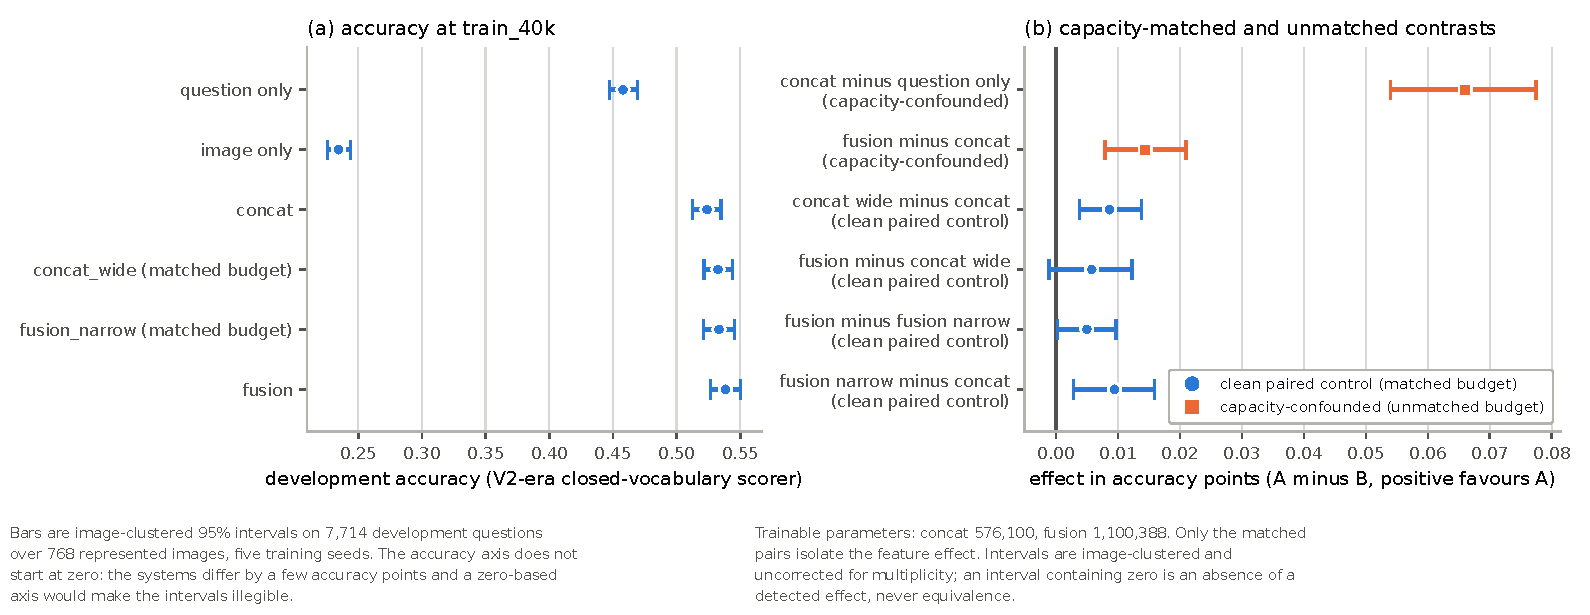
\includegraphics[width=\textwidth]{ve1/VE1-FIG-02.pdf}
\caption[Low-data ladder with capacity controls.]{Low-data accuracy and paired contrasts on 7,714 development questions over 768 represented images. Intervals are nominal image-clustered evaluation-sampling intervals. The unmatched fusion--concatenation comparison is capacity-confounded; only the matched pairs isolate the feature change, and one matched interval includes zero.}
\label{fig:ch4-ladder}
\end{figure}

\section{Visual reliance}
\label{sec:ch4-reliance}
The visual-reliance experiment changed the image input while leaving each
question unchanged. In v2\_06, image embeddings were either permuted across
development rows or replaced by zeros. The row-level permutation contained 11
self-pairs, or 0.14\% of rows, which slightly dilutes the shuffled
intervention. This is the controlling intervention generation for RQ1.

Figure~\ref{fig:ch4-reliance} shows the drops on the 7,714-row top-100 view.
Fusion dropped by 0.14270 under shuffled images and 0.11880 under zeroed images,
with intervals [0.12769, 0.15759] and [0.10403, 0.13305]. The corresponding
drops for concatenation were 0.11709 [0.10295, 0.13035] and 0.09987 [0.08697,
0.11228]. The matched-budget product head lay between them. The question-only
control had an exact zero drop under both interventions by construction.

The multimodal heads therefore depend on receiving the correct image. This
does not establish visual grounding, compositional reasoning, causal reasoning
or human-like understanding; the intervention measures dependence only.

The two interventions answer related but different questions. Shuffling asks
whether the head needs the image paired with the question rather than another
development image. Zeroing asks whether its prediction changes when the image
representation is removed. Their drop sizes are not treated as a decomposition
of visual information, and neither intervention identifies the reasoning
process used to produce an answer.

\begin{figure}[p]
\centering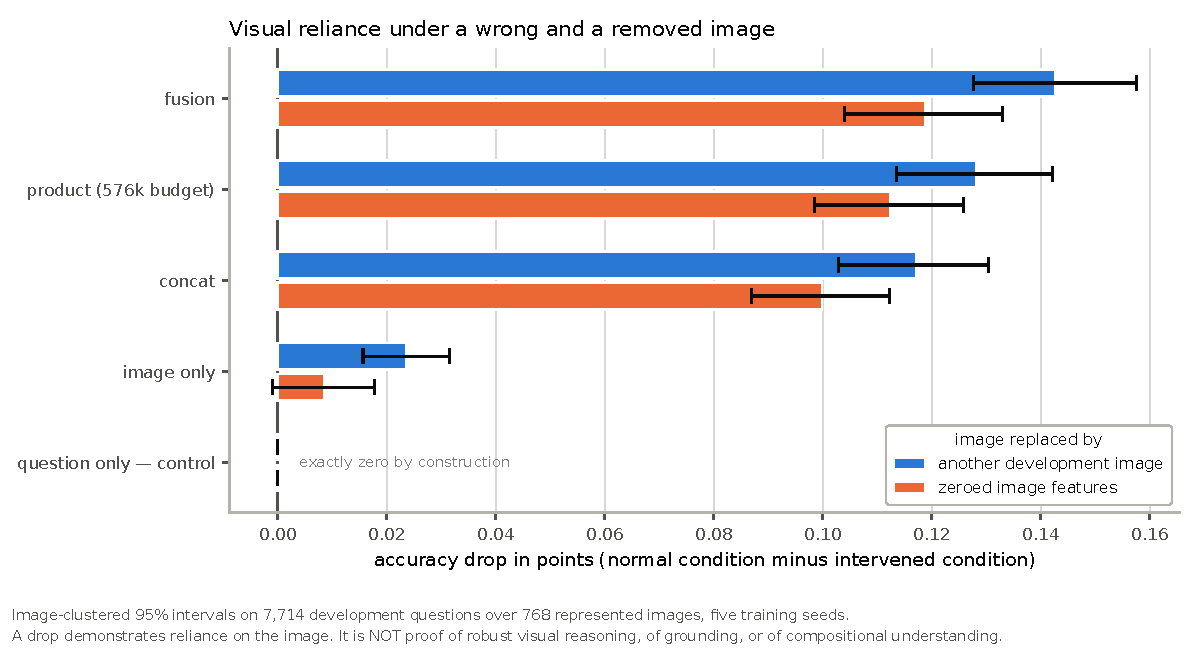
\includegraphics[width=\textwidth]{ve1/VE1-FIG-05.pdf}
\caption[Visual reliance under wrong and removed images.]{Accuracy drops on 7,714 development questions when the image is replaced or removed. Intervals are nominal image-clustered intervals. Question only is exactly zero by construction and is a control. A drop demonstrates dependence on the correct image, not robust visual reasoning, grounding or compositional understanding.}
\label{fig:ch4-reliance}
\end{figure}

\section{Training scale}
\label{sec:ch4-scaling}
Figure~\ref{fig:ch4-scaling} follows four heads across 40k, 100k and 250k
labelled questions on the 7,714-row top-100 view. Fusion moved from 0.53840 to
0.56308 and 0.58226; concatenation moved from 0.52398 to 0.55084 and 0.57861.
The matched product head reached 0.53355, 0.56365 and 0.58242, while question
only rose from 0.45797 to 0.48294 and 0.49769. Every stored series therefore
increased across the three scales.

The fusion-minus-concatenation difference narrowed from +0.01442 at 40k to a
seed-mean difference of +0.00365 at 250k. Seeds 2 and 42 reversed its direction
at 250k. No image-clustered interval is available for v2\_07, and the figure's
error bars are sample SD across training seeds rather than confidence
intervals. The narrowing is therefore tentative, not statistically
established. Three training sizes also do not support a general scaling law.

The consistent rise in the stored means supports only a result about the three
tested training sizes. It does not show how the heads would behave between or
beyond them. Likewise, the smaller fusion--concatenation gap at the largest
scale is descriptive because its uncertainty is represented only by variation
between training seeds. This limitation is why the scaling claim remains
tentative even though the plotted means are ordered clearly.

\begin{figure}[p]
\centering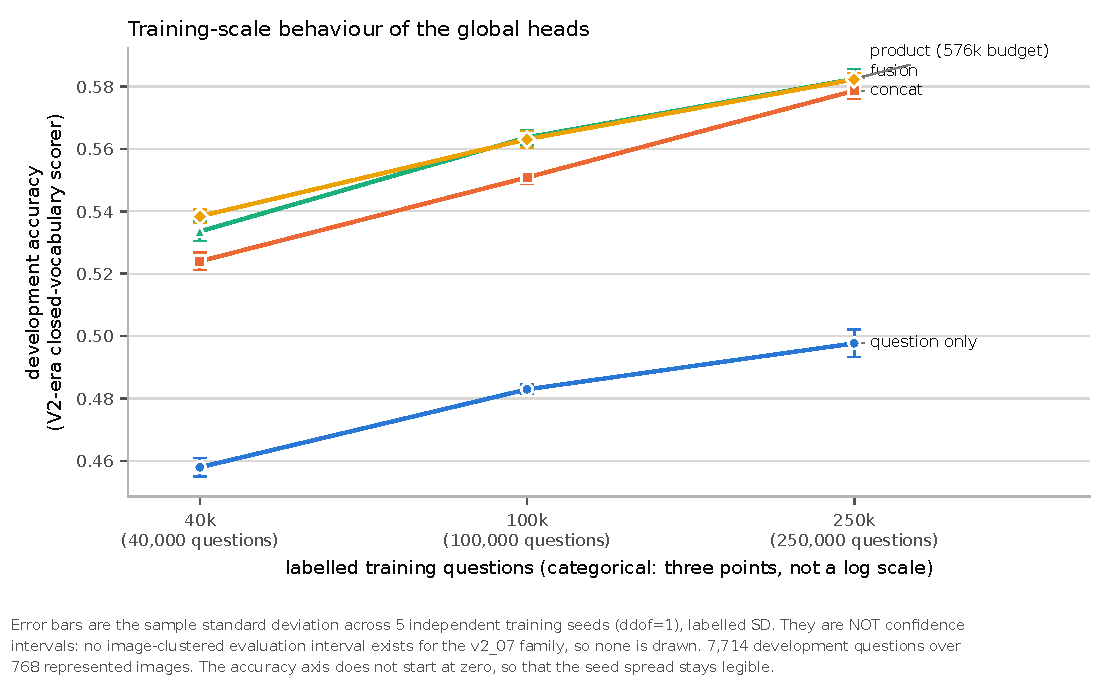
\includegraphics[width=\textwidth]{ve1/VE1-FIG-03.pdf}
\caption[Training-scale behaviour of the global heads.]{Top-100 development accuracy across 40k, 100k and 250k labelled questions. Error bars are the sample standard deviation across five training seeds (\texttt{ddof=1}); they are not confidence intervals. Under the accepted v2\_07 limitation, no image-clustered interval exists for this family, so the 250k narrowing remains tentative.}
\label{fig:ch4-scaling}
\end{figure}

\section{Representation quality}
\label{sec:ch4-representation}
The primary encoder comparison replaces CLIP with SigLIP while retaining the
40k recipe and the same 7,714 development rows. Figure~\ref{fig:ch4-encoder}
shows SigLIP-minus-CLIP differences of +0.01540 for concatenation, +0.01475 for
fusion and +0.01356 for product. Their intervals are [0.00592, 0.02481],
[0.00601, 0.02401] and [0.00403, 0.02282], all excluding zero. The
question-only difference was +0.00814 with interval [-0.00006, 0.01586], which
includes zero. The stronger multimodal pattern supports representation quality
as an important factor acting mainly through the image path in this experiment.

The comparison is REPRESENTATION\_CONFOUNDED. Encoder identity, embedding
width (512 for CLIP and 768 for SigLIP) and head input width change together.
The development rows match, but training streams are not paired by seed. The
result therefore isolates neither a pure encoder effect nor a single determining constraint.

The cleanest conclusion is therefore limited to the tested encoder systems at
40k. On identical evaluation rows, the multimodal SigLIP systems have positive
contrasts whose intervals exclude zero. The question-only contrast is not
resolved clearly by its interval. This pattern is consistent with an important
image-side representation difference, but the simultaneous width changes stop
it from identifying the encoder alone as the cause.

At 250k on the same 7,714-row view, the stored five-seed SigLIP means were
0.59388 for fusion, 0.59176 for concatenation and 0.50236 for question only,
with seed SDs 0.00317, 0.00261 and 0.00449. No clustered
SigLIP-minus-CLIP interval exists at this scale. As descriptive cross-family
context only, the five-seed SigLIP fusion mean of 0.59388 is comparable to the
three-seed, 21.1M-parameter latent reasoner mean of 0.59580 on that development
view. The capacity-mismatched SigLIP product reference is excluded.

The reasoner comparison is deliberately secondary. It places the stored means
on a common descriptive accuracy scale, but it does not hold architecture,
input granularity, trainable capacity or seed structure fixed. No clustered
contrast connects the two families at this scale. The observation can therefore
show that the values are comparable, but not that one architecture has been
shown to outperform the other.

\begin{figure}[p]
\centering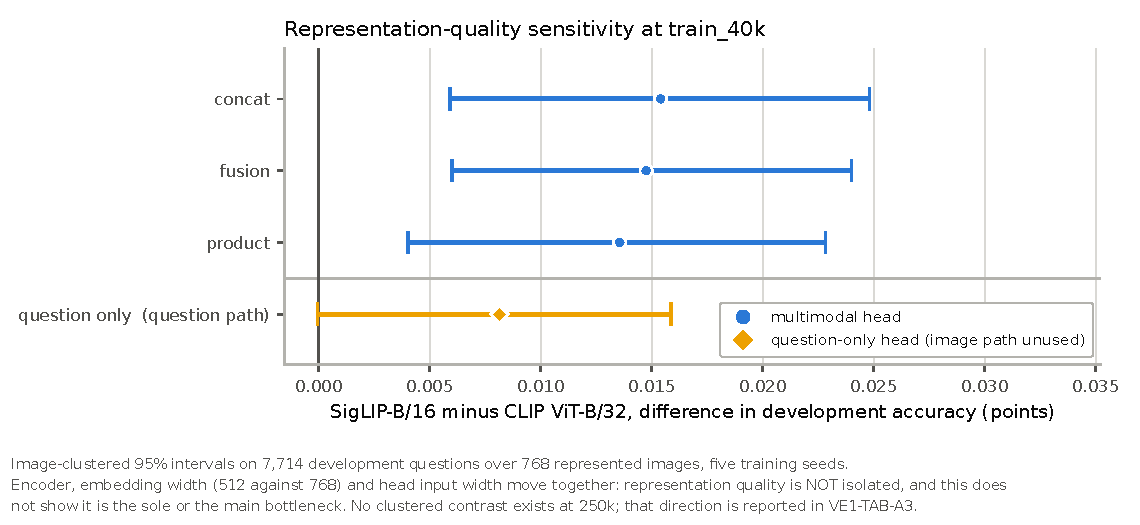
\includegraphics[width=\textwidth]{ve1/VE1-FIG-07.pdf}
\caption[Representation sensitivity at 40k.]{SigLIP-minus-CLIP differences on the same 7,714 development rows. Intervals are nominal image-clustered intervals. Representation is not isolated: encoder identity, embedding width and head input width move together, training streams are not seed-paired, and no clustered contrast exists at 250k.}
\label{fig:ch4-encoder}
\end{figure}

\section{Answer-set size}
\label{sec:ch4-answer-space}
Expanding the vocabulary changes both coverage and the classification problem.
Top-100 coverage is 0.77109 of the shared 10,004-question development
distribution; top-1000 coverage is 0.98191. The top-1000 view therefore has
9,823 questions over 776 images rather than the top-100 view's 7,714 questions
over 768 images.

At 250k, top-1000 in-vocabulary accuracies were 0.40625 for question only,
0.49111 for concatenation, 0.49946 for product and 0.49547 for fusion. Their
intervals in Table~\ref{tab:ch4-answer-space} apply only to the 9,823-row view.
Within that view, fusion minus concatenation was +0.00436 with interval
[-0.00138, 0.00995], so the contrast is not resolved clearly.

The derived raw-distribution column places results on the shared 10,004-row
distribution by multiplying stored in-vocabulary accuracy by coverage. It
gives 0.4490 for top-100 fusion and 0.4462 for top-100 concatenation, compared
with 0.4866 and 0.4822 for their top-1000 counterparts; top-1000 product reaches
0.4905. These are labelled derived quantities, not cross-vocabulary accuracy
contrasts. The in-vocabulary values are never subtracted because answer sets,
training rows and denominators differ. The seed-0 shared-head diagnostic is
omitted because it is not like-for-like with the five-seed top-100 mean.

Coverage and in-vocabulary accuracy answer different questions. Coverage asks
how much of the raw development distribution is represented by an answer
vocabulary. In-vocabulary accuracy asks how often the system is correct after
restricting evaluation to those represented answers. The derived column gives
a row-fair view by placing the stored values back on the shared raw
distribution. It is useful for comparing coverage--accuracy trade-offs, but it
does not turn the two classifier tasks into a paired experiment.

Table~\ref{tab:ch4-answer-space} leaves the question-only derived entry blank
because the controlling report does not state that value. No value is inferred
to fill the presentation. This keeps the table tied to the frozen record and
prevents a convenient arithmetic extension from becoming new evidence.

\begin{table}[p]
\centering
\caption[Answer-space size and development coverage.]{Top-100 and top-1000 results at 250k with distinct in-vocabulary denominators. The raw-distribution column copies the E3 report's derived values on the shared 10,004-row distribution. In-vocabulary accuracies are never differenced across answer spaces.}
\label{tab:ch4-answer-space}
\begingroup\tiny\setlength{\tabcolsep}{1.2pt}
\renewenvironment{longtable}[1]{\begin{tabular}{|p{0.09\textwidth}|p{0.11\textwidth}|p{0.12\textwidth}|p{0.14\textwidth}|p{0.20\textwidth}|p{0.09\textwidth}|p{0.17\textwidth}|}}{\end{tabular}}
\let\endhead\relax\renewcommand{\_}{\textunderscore\allowbreak}
% Generated by tools/tab2latex.py; do not edit.
% Presentation metadata: {"header_map":{"95% CI (image-clustered)":"Image-clustered 95% CI","answer space":"Answer space","coverage":"Coverage","denominator":"Development denominator","derived raw-distribution accuracy":"Derived raw-distribution accuracy","in-vocabulary accuracy":"In-vocabulary accuracy","system":"System"},"source_headers":["answer space","system","denominator","in-vocabulary accuracy","95% CI (image-clustered)","coverage","derived raw-distribution accuracy"],"thousands":false}
\begin{longtable}{|l|l|l|l|l|l|l|}
\hline
Answer space & System & Development denominator & In-vocabulary accuracy & Image-clustered 95\% CI & Coverage & Derived raw-distribution accuracy \\ \hline
\endhead
top-100 & concat & 7,714 & 0.57861 & not available & 0.77109 & 0.4462 \\ \hline
top-100 & fusion & 7,714 & 0.58226 & not available & 0.77109 & 0.4490 \\ \hline
top-1000 & question\_only & 9,823 & 0.40625 & [0.39630, 0.41655] & 0.98191 &  \\ \hline
top-1000 & concat & 9,823 & 0.49111 & [0.47957, 0.50229] & 0.98191 & 0.4822 \\ \hline
top-1000 & product & 9,823 & 0.49946 & [0.48765, 0.51060] & 0.98191 & 0.4905 \\ \hline
top-1000 & fusion & 9,823 & 0.49547 & [0.48321, 0.50775] & 0.98191 & 0.4866 \\ \hline
\end{longtable}

\endgroup
\end{table}

\section{RQ1 summary}
\label{sec:ch4-summary}
On the 7,714-row top-100 development view, lightweight heads over frozen
global representations answer the closed-set task well above either unimodal
reference. At 40k,
explicit interactions improve over concatenation, with an interval excluding
zero and the same direction in every seed. Matched controls narrow the claim:
capacity explains part of the gain, while the lower-budget comparison retains
evidence for the feature change. The multimodal systems also depend on the
correct image.

More labelled questions improve every tested head, although the fusion
advantage narrows at 250k without a clustered interval. The paired 40k encoder
comparison supports representation quality as an important but confounded
factor; at 250k SigLIP fusion is descriptively comparable to the larger
reasoner. The 1,000-answer vocabulary raises coverage and derived
raw-distribution accuracy while defining a different in-vocabulary task.
Chapter~8 considers the broader interpretation and limits of these
development-set findings.

Several stronger conclusions are not established. The evidence does not show
that interaction is generally better than capacity, that representation alone
determines performance, or that the fusion advantage follows a scaling law.
The cross-family context establishes no advantage for SigLIP fusion over the
reasoner, and
the reliance interventions do not establish grounding or compositional
reasoning. Finally, all findings remain development-set results; they provide
no held-out or clean-test conclusion.

\fussy

\chapter{RQ2 — Latent Reasoning and Compositional Difficulty}
% TODO Phase 1 (dissertation-05): sources per docs/DISSERTATION_HANDOFF.md; internal budget 1900 words; stub only in Phase 0.

\chapter{RQ3 — Frozen Small-Language-Model Interfaces}
% TODO Phase 1 (dissertation-06): sources per docs/DISSERTATION_HANDOFF.md; internal budget 1900 words; stub only in Phase 0.

\chapter{Efficiency and Accuracy–Efficiency Trade-offs}

\section{Scope and measurement boundary}
\label{sec:ch7-scope}

This chapter reports computational efficiency for the development systems
examined in Chapters 4--6. The headline latency evidence is the final E7b
serial experiment described in Section~\ref{sec:ch3-efficiency}. It measures a
complete batch-1 query in fp32 on an NVIDIA RTX 4000 Ada GPU on node
\texttt{otter155}. Each system was run in a fresh subprocess in each of three
pass-major runs, using a pinned random order. Each run used 50 warm-up queries
followed by 300 timed queries, with device synchronisation around each call.
The headline quantity is the median warm-query latency. It is a measured time,
not a confidence interval.

The end-to-end boundary starts with reading the image file and ends with
decoding the predicted answer. Depending on the interface, it includes CPU
decode and preprocessing, host-to-device transfer, the frozen vision tower,
question tokenisation, a frozen text or language-model tower, trainable
projection, fusion or latent reasoning, classification and answer decoding.
Cached-feature and head-only timings therefore answer a different question and
are not treated as end-to-end results. The earlier E7a additive pipeline sums
and their frontiers are superseded. E7b cold-first-query latency and peak-memory
fields are withdrawn without replacement and are omitted here.

All accuracies are development results. The timed E7b checkpoints are seed-0
checkpoints trained on 250k questions, so their accuracy values are frozen
single-checkpoint results rather than the multi-seed means used elsewhere.
Energy, power, carbon and monetary cost were not measured, so no claim is made
about those quantities.

\section{Warm-serial latency on the E7b node}
\label{sec:ch7-latency}

Table~\ref{tab:ch7-e7b} reports the eight governed E7b systems. The
question-only pipeline is a labelled non-multimodal floor at 1.9603 ms. The
three global multimodal heads occupy a narrow band: concat takes 7.6104 ms,
fusion 7.6351 ms and the top-1000 product head 7.6708 ms. Their across-pass
spreads are 0.9044, 0.8903 and 0.0966 ms respectively. These measurements
include their frozen encoder paths rather than only the small trainable heads.
The three rows remain distinct implemented pipelines, even though their warm
medians are close. Across-pass spread is the maximum difference among the
three pass summaries. It supplies repeatability context for the timing runs;
it is neither an evaluation-sampling interval nor a test that two systems
have equal latency.

Token-level interfaces take longer under the same protocol. The latent
reasoner records 9.1719 ms and the CLIP-token A0p interface 9.2117 ms. The
SigLIP fusion system records 9.8433 ms, while the question-side SmolLM2 A1
interface records 20.1460 ms. Across-pass spread ranges from 0.0770 ms for
SigLIP fusion to 1.3302 ms for A1. This ordering is specific to the stated
hardware, checkpoints and serial protocol; it is not inferred from parameter
counts.

The ordering also depends on what is included in the measurement. For
example, the question-only floor omits an image path, whereas every governed
multimodal row includes image loading, preprocessing and its frozen vision
tower. It is therefore useful as a labelled lower boundary for the complete
pipeline, but it is not evidence that removing vision is an acceptable
substitute for a multimodal system.

\begin{table}[p]
\centering
\caption[E7b serial latency, accuracy and parameter counts.]{Seed-0 250k development checkpoints under the E7b end-to-end serial protocol on \texttt{otter155}. Supported-view accuracy uses the answer space shown and is not a common metric across the top-100 and top-1000 rows. Raw-distribution accuracy uses the common 10,004-row view. The canonical frontier uses only that raw accuracy and warm median latency; question only is excluded as a non-multimodal floor. Medians and across-pass spreads are latency summaries, not confidence intervals.}
\label{tab:ch7-e7b}
\begingroup\scriptsize\setlength{\tabcolsep}{0.55pt}
\makeatletter
\let\chSevenArrayParboxRestore\@arrayparboxrestore
\def\@arrayparboxrestore{\chSevenArrayParboxRestore\raggedright\let\\\tabularnewline}
\makeatother
\renewenvironment{longtable}[1]{\begin{tabular}{|p{0.12\textwidth}|p{0.105\textwidth}|p{0.078\textwidth}|p{0.078\textwidth}|p{0.076\textwidth}|p{0.062\textwidth}|p{0.10\textwidth}|p{0.115\textwidth}|p{0.075\textwidth}|}}{\end{tabular}}
\let\endhead\relax\renewcommand{\_}{\textunderscore\allowbreak}
% Generated by tools/tab2latex.py; do not edit.
% Presentation metadata: {"header_map":{"answer view":"Answer view","frontier":"Frontier","raw accuracy (10,004)":"Raw accuracy (10,004)","spread ms":"Spread (ms)","supported accuracy":"Supported accuracy","system":"System","total loaded parameters":"Total loaded parameters","trainable parameters":"Trainable parameters","warm median ms":"Warm median (ms)"},"source_headers":["system","answer view","supported accuracy","raw accuracy (10,004)","warm median ms","spread ms","trainable parameters","total loaded parameters","frontier"],"thousands":true}
\begin{longtable}{|l|l|l|l|l|l|l|l|l|}
\hline
System & Answer view & Supported accuracy & Raw accuracy (10,004) & Warm median (ms) & Spread (ms) & Trainable parameters & Total loaded parameters & Frontier \\ \hline
\endhead
Question only & top-100 (7,714) & 0.50402 & 0.38864 & 1.9603 & 0.0133 & 313,956 & 151,591,269 & excluded floor \\ \hline
Concat & top-100 (7,714) & 0.57661 & 0.44462 & 7.6104 & 0.9044 & 576,100 & 151,853,413 & yes \\ \hline
Fusion & top-100 (7,714) & 0.58439 & 0.45062 & 7.6351 & 0.8903 & 1,100,388 & 152,377,701 & yes \\ \hline
Top-1000 product & top-1000 (9,823) & 0.49954 & 0.49050 & 7.6708 & 0.0966 & 1,299,944 & 152,577,257 & yes \\ \hline
Latent reasoner & top-100 (7,714) & 0.59139 & 0.45602 & 9.1719 & 0.9211 & 21,099,620 & 172,376,933 & no \\ \hline
CLIP-token A0p & top-100 (7,714) & 0.59463 & 0.45852 & 9.2117 & 0.1367 & 21,362,276 & 172,639,589 & no \\ \hline
SigLIP fusion & top-100 (7,714) & 0.59386 & 0.45792 & 9.8433 & 0.0770 & 1,624,676 & 204,780,646 & no \\ \hline
SmolLM2 A1 & top-100 (7,714) & 0.57493 & 0.44332 & 20.1460 & 1.3302 & 21,395,044 & 307,187,365 & no \\ \hline
\end{longtable}

\endgroup
\end{table}

\section{Accuracy--latency frontier}
\label{sec:ch7-frontier}

The accuracy columns in Table~\ref{tab:ch7-e7b} preserve two denominator
conventions. Top-100 systems are evaluated on 7,714 supported questions,
whereas the top-1000 product head is evaluated on 9,823 supported questions.
Those supported-view accuracies are not compared across vocabularies. The
frontier instead uses raw-distribution accuracy on the common 10,004-row
development view, following the scoring distinction in
Section~\ref{sec:ch3-scoring} and the answer-space analysis in
Section~\ref{sec:ch4-answer-space}.

On this common axis, the canonical E7b frontier contains concat, fusion and
the top-1000 product head. Their raw-distribution accuracies are 0.44462,
0.45062 and 0.49050. The corresponding warm serial medians are 7.6104,
7.6351 and 7.6708 ms on \texttt{otter155}. Question only is excluded from
frontier construction because it is not a multimodal system. Among the
multimodal systems included in the canonical E7b frontier analysis, the latent
reasoner, A0p, SigLIP fusion and A1 are dominated. This is a two-axis result:
trainable and total loaded parameter counts are descriptive columns, not
Pareto axes.

In the retained frontier record, a multimodal point is dominated when another
included multimodal system has no lower raw-distribution accuracy and no
higher latency, with at least one strict improvement. The label consequently
applies only to the two plotted quantities. It does not rank supported-view
accuracy, trainable capacity or loaded parameter count. In particular, the
top-1000 product point occupies the high-accuracy end of the frontier because
of its common-view raw accuracy; its top-1000 supported-view value is not
compared directly with the top-100 supported values.

Figure~\ref{fig:ch7-efficiency} retains the two-node presentation used by the
frozen evidence layer. The panels cannot be merged because the shared fusion
bridge differed by the stored $-18.69\%$ against a pre-registered
$\pm10\%$ gate. The bridge therefore failed, and no adjustment factor is
applied.

\begin{figure}[p]
\centering
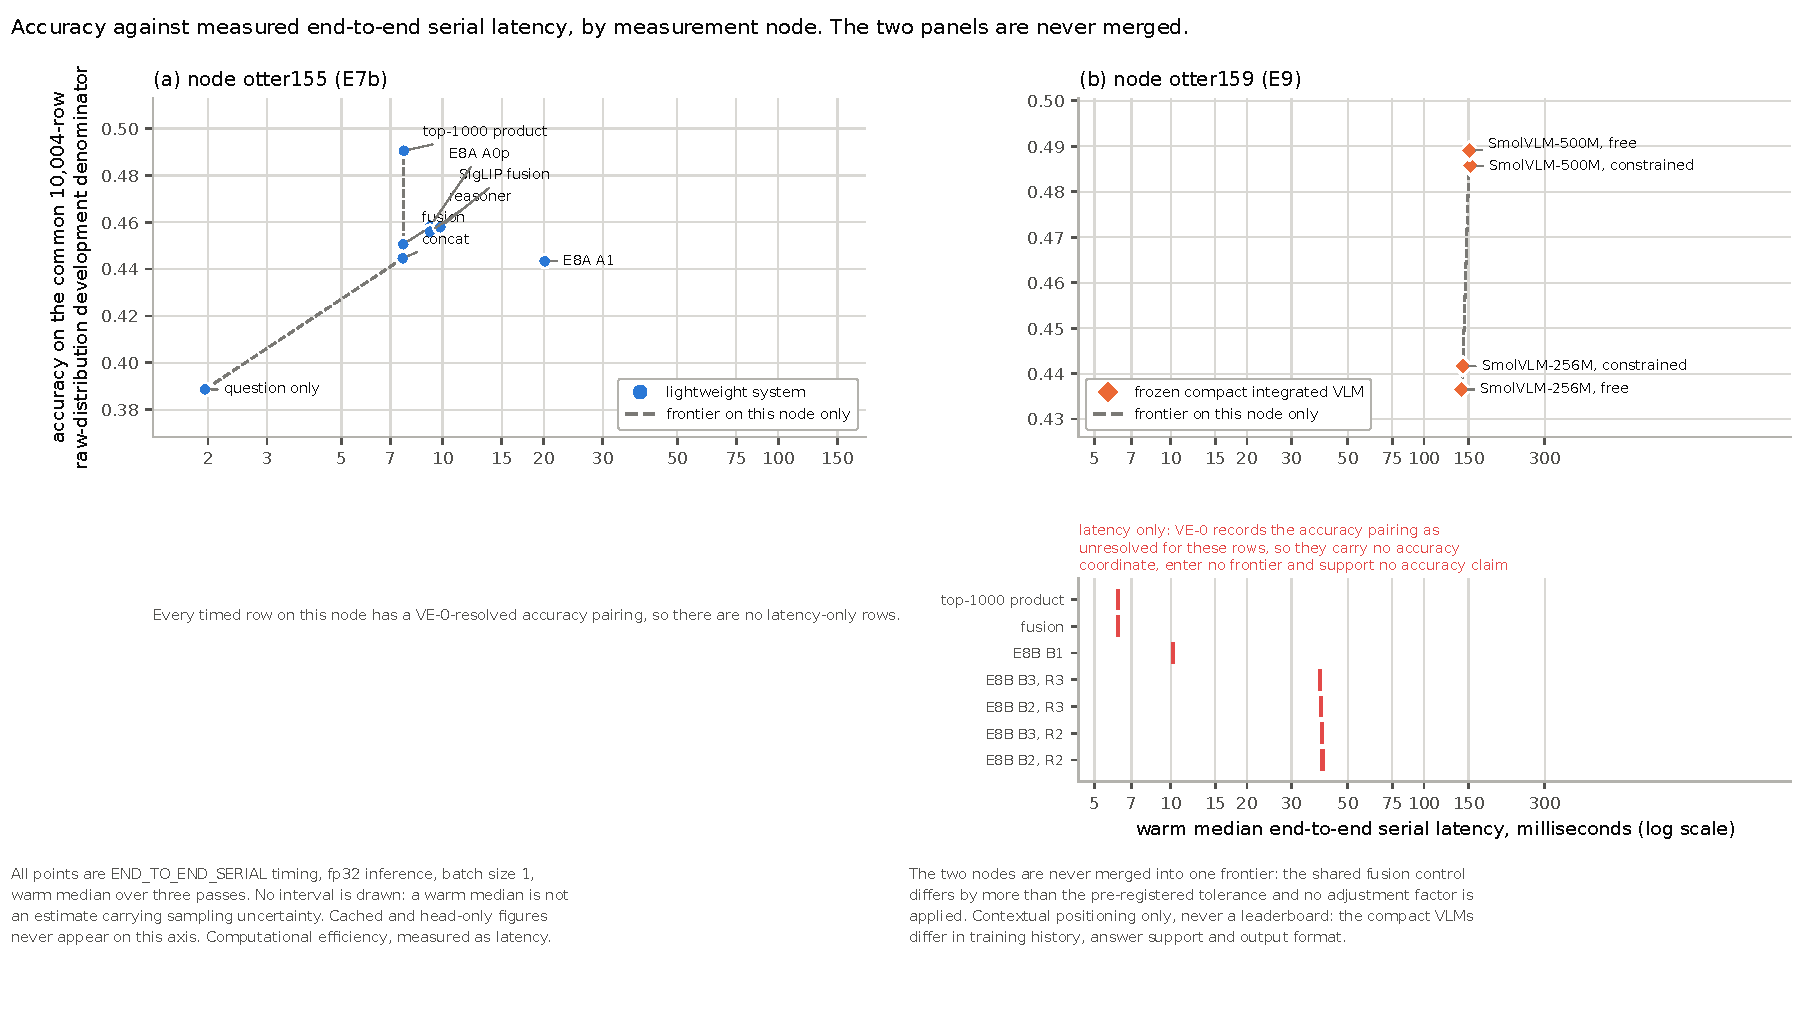
\includegraphics[width=0.98\textwidth]{images/ve1/VE1-FIG-09.pdf}
\caption[Accuracy against warm serial latency by node.]{Development accuracy against measured end-to-end warm serial latency, with \texttt{otter155} and \texttt{otter159} kept in separate panels. The fusion bridge differed by $-18.69\%$ against the $\pm10\%$ gate, so the nodes are never merged and no adjustment factor is used. Only end-to-end serial rows are shown: cached/head-only timings are not treated as end-to-end, and E7a additive sums are superseded. E9 is contextual and its unresolved reference rows are latency-only. E10 has no timing evidence. The figure supports computational latency claims only; it provides no energy, power, carbon or monetary-cost measurement.}
\label{fig:ch7-efficiency}
\end{figure}

\section{Parameter counts and interface cost}
\label{sec:ch7-parameters}

Table~\ref{tab:ch7-e7b} reports trainable parameter count separately from total
loaded parameter count. The former describes optimised capacity. The latter
counts parameters resident in the measured system under the E7b convention;
it is not checkpoint storage, file size, VRAM or a measured memory footprint.
Nominal labels such as 135M and 500M identify model families and should not be
read as trainable counts.

The global heads have between 576,100 and 1,624,676 trainable parameters in
the multimodal rows, while the latent reasoner, A0p and A1 have between
21,099,620 and 21,395,044. Their total loaded counts also differ because the
resident frozen towers differ. These counts establish capacity and residency
context, but they do not predict the observed latency ordering. No parameter
ratio is used as an efficiency result.

The answer-side timing boundary is narrower still. E9 times B1 and the B2/B3
R2 and R3 generation readouts on \texttt{otter159}. No serial latency was
measured for the Chapter-6 R1 likelihood readout, and R2/R3 timings are not its
cost. B4, B4r and E10 were not measured under a valid comparable headline
timing protocol. Parameter count alone is not used to fill these missing
measurements.

The retained segmented pass gives limited attribution context, while remaining
separate from the headline measurement. In that pass, the reasoner block takes
1.8014 ms, the SigLIP vision tower 4.9889 ms and the A1 SmolLM2 forward pass
13.4581 ms. These are segmented-pass components, not end-to-end latencies, and
they are not added to construct an alternative pipeline total. They describe
where time was observed within those instrumented passes without establishing
why one interface takes longer.

\section{Same-node compact-VLM context}
\label{sec:ch7-vlm}

Table~\ref{tab:ch7-e9} reports the E9 timing block on \texttt{otter159}, using
the imported serial harness with batch 1, 50 warm-up queries, 300 timed queries
and three passes. It is contextual evidence on a separate node, not an
extension of the E7b frontier. The re-timed top-1000 product head records
6.1990 ms under this timing protocol. The E9 artefact does not restate the
checkpoint identity for that row, so its accuracy is deliberately unavailable
in Table~\ref{tab:ch7-e9}.

Separately, the canonical development record gives the top-1000 product
system a common-view raw accuracy of 0.49050 on 10,004 rows. These facts are
not combined into a paired E9 coordinate. E9 does pair the SmolVLM rows with
their own G21 raw-distribution accuracies: the 256M
family records 0.436525 open and 0.441623 constrained, with latencies 140.9070
and 142.6747 ms; the 500M family records 0.489004 open and 0.485706
constrained, with latencies 151.3801 and 152.8540 ms.

The open rows use free greedy generation capped at 20 tokens. The constrained
rows use greedy decoding masked to the top-1000 answer-prefix trie. Both are
retained because they are paired E9 measurements, but the constrained readout
is a secondary diagnostic rather than a replacement accuracy protocol. The
B1 and B2/B3 rows in the same table are latency-only context: their missing
accuracy coordinates preserve the same unresolved-pairing boundary as the
re-timed head rows.

The canonical stored latency statement is that SmolVLM-500M constrained was
approximately 24.7 times slower in warm serial latency than the re-timed head
under the same-node contextual protocol. This statement compares latency only.
It does not create a paired accuracy comparison, a leaderboard or a general
claim about compact VLMs. The fusion bridge row is 6.2081 ms, but its failed
cross-node gate prevents any merge with the 7.6351 ms E7b fusion result.

\begin{table}[p]
\centering
\caption[E9 same-node timing context.]{Warm serial development timing on \texttt{otter159} under the E7b harness imported read-only. The block is contextual only: the fusion bridge failed, nodes are not merged, and no adjustment factor is used. Accuracy is shown only for the four canonically paired SmolVLM rows; re-timed product, fusion and B1/B2/B3 rows remain explicitly unpaired. No R1 answer-side latency exists, R2/R3 timings are not R1 cost, and E10 has no timing evidence.}
\label{tab:ch7-e9}
\begingroup\scriptsize\setlength{\tabcolsep}{0.65pt}
\makeatletter
\let\chSevenArrayParboxRestoreB\@arrayparboxrestore
\def\@arrayparboxrestore{\chSevenArrayParboxRestoreB\raggedright\let\\\tabularnewline}
\makeatother
\renewenvironment{longtable}[1]{\begin{tabular}{|p{0.14\textwidth}|p{0.15\textwidth}|p{0.10\textwidth}|p{0.115\textwidth}|p{0.085\textwidth}|p{0.07\textwidth}|p{0.10\textwidth}|p{0.07\textwidth}|}}{\end{tabular}}
\let\endhead\relax\renewcommand{\_}{\textunderscore\allowbreak}
% Generated by tools/tab2latex.py; do not edit.
% Presentation metadata: {"header_map":{"paired E9 raw accuracy":"Paired E9 raw accuracy","pairing status":"Pairing","role or readout":"Role or readout","spread ms":"Spread (ms)","system":"System","total loaded parameters":"Total loaded parameters","trainable parameters":"Trainable parameters","warm median ms":"Warm median (ms)"},"source_headers":["system","role or readout","trainable parameters","total loaded parameters","warm median ms","spread ms","paired E9 raw accuracy","pairing status"],"thousands":true}
\begin{longtable}{|l|l|l|l|l|l|l|l|}
\hline
System & Role or readout & Trainable parameters & Total loaded parameters & Warm median (ms) & Spread (ms) & Paired E9 raw accuracy & Pairing \\ \hline
\endhead
Top-1000 product & re-timed product head & 1,299,944 & 152,577,257 & 6.1990 & 0.0827 & unavailable & unpaired \\ \hline
Fusion bridge & cross-node bridge control & 1,100,388 & 152,377,701 & 6.2081 & 0.0179 & unavailable & unpaired \\ \hline
B1 classifier & LM-free classifier & 21,100,132 & 172,377,445 & 10.2420 & 0.4224 & unavailable & unpaired \\ \hline
B2 R2 & random 135M, constrained & 21,343,808 & 307,136,129 & 39.7326 & 1.4689 & unavailable & unpaired \\ \hline
B2 R3 & random 135M, open & 21,343,808 & 307,136,129 & 39.2394 & 1.2055 & unavailable & unpaired \\ \hline
B3 R2 & pretrained 135M, constrained & 21,343,808 & 307,136,129 & 39.6561 & 0.4844 & unavailable & unpaired \\ \hline
B3 R3 & pretrained 135M, open & 21,343,808 & 307,136,129 & 38.7963 & 0.3720 & unavailable & unpaired \\ \hline
SmolVLM-256M open & primary open generation & 0 & 256,484,928 & 140.9070 & 1.3031 & 0.436525 & resolved \\ \hline
SmolVLM-256M constrained & constrained diagnostic & 0 & 256,484,928 & 142.6747 & 0.7703 & 0.441623 & resolved \\ \hline
SmolVLM-500M open & primary open generation & 0 & 507,482,304 & 151.3801 & 1.2941 & 0.489004 & resolved \\ \hline
SmolVLM-500M constrained & constrained diagnostic & 0 & 507,482,304 & 152.8540 & 1.2409 & 0.485706 & resolved \\ \hline
\end{longtable}

\endgroup
\end{table}

% XREF-PENDING: appendix figure VE1-FIG-A5

\clearpage
\section{Efficiency summary}
\label{sec:ch7-summary}

Under the E7b protocol, the global multimodal heads occupy the lowest-latency
part of the governed multimodal set, at 7.6104--7.6708 ms, while the token-level
interfaces range from 9.1719 to 20.1460 ms. On the common 10,004-row
raw-distribution axis, concat, fusion and the top-1000 product head form the
canonical accuracy--latency frontier. The result is bounded to seed-0 250k
development checkpoints, otter155 and the stated serial measurement contract.

The E9 block gives separate same-node context for compact VLMs on otter159.
Its paired SmolVLM accuracies and latencies do not resolve the checkpoint
pairing of the re-timed product-head row, and the failed bridge prevents
cross-node merging. Accordingly, Chapter 7 supports claims about measured
warm serial latency, trainable parameter count and total loaded parameter
count only. Peak memory, storage size and environmental or monetary quantities
remain outside the retained evidence. No held-out inference follows from
these development measurements. Broader interpretation and design
implications are deferred to Chapter 8.

\chapter{Discussion}

\section{Overall interpretation}
\label{sec:ch8-overall}

The results support a bounded account of efficient closed-set VQA on this GQA
development partition. Compact trainable heads can use frozen representations
to combine strong question-side predictive information with a real visual
contribution. At 40k, the question-only head reaches 0.45797 and fusion reaches
0.53840. The intervention evidence then shows that the multimodal heads depend
on receiving the correct image; it does not establish visual grounding or
reasoning. This use of frozen features with a small closed-answer classifier
has precedent on a different VQA setting \citep{deuser2022less}, but the
dataset and protocol differences preclude a numerical comparison.

Across the implemented systems, representation choice, interaction design and
answer-space coverage all materially affect the observed results. Additional
downstream capacity alone does not consistently explain the strongest
configurations. This is not a global ranking of those design choices: the
top-100 and top-1000 evaluations define different supported-answer tasks, and
cross-family comparisons often change several factors together. The following
sections therefore interpret the controlled contrasts first and use the less
closely matched comparisons only as qualified context.

\section{Representations, interaction and latent reasoning}
\label{sec:ch8-representation}

The RQ1 evidence gives explicit interaction a clear but limited role. Fusion
exceeds concatenation by +0.01442 at 40k, yet the capacity controls show that
part of this difference follows from the wider head. At the larger matched
budget, the fusion-minus-concat-wide effect is +0.00578 with interval
$[-0.00116,0.01226]$, so that residual contrast is not resolved clearly.
This separation of interaction from an additive approximation is conceptually
related to the question posed by EMAP \citep{hessel2020emap}; here it is tested
constructively with capacity controls. The later narrowing of the
fusion--concatenation gap remains descriptive because no clustered interval is
available for that scaling family.

Representation choice also matters, but the encoder comparison is not
factorial. At 250k, SigLIP fusion at 0.59388 is descriptively competitive with
the latent reasoner at 0.59580 in the tested configurations.
Encoder and interface widths, architecture and other configuration details
co-vary, and the seed structures differ. The observation is therefore neither
a paired causal comparison nor evidence that a stronger representation can
generally replace downstream reasoning capacity.

The reasoner's overall accuracy rises across the tested scales, and its
same-seed advantage over fusion is positive in every stored seed at the two
larger scales. This remains configuration-level evidence because architecture,
token access and capacity change together. Learned latent bottlenecks have
architectural precedents in Perceiver and BLIP-2
\citep{jaegle2021perceiver,li2023blip2}, but those lineages do not identify the
source of this project's accuracy pattern. More importantly, the fixed-prior
four-or-more-step deficit persists and its paired difference from fusion is
unresolved at every tested scale. The implemented changes did not eliminate
that profile, but they do not localise its cause.

The question-only result provides an internal check on what this statistic
means. At the largest scale it has a smaller pooled deficit than the
multimodal systems despite substantially lower overall accuracy. A lower
deficit therefore describes a less uneven fixed-prior step profile, not a
better model or stronger reasoning ability. Conversely, the reasoner's higher
overall accuracy at the larger scales does not establish that its persistent
multi-step difficulty has been removed.

That restraint is consistent with the wider evidence base. Binding information
can remain linearly accessible in unimodal CLIP features
\citep{koishigarina2026bow}, while work with much larger decoders locates
feature-use limitations differently or finds compensation for degraded visual
context \citep{fu2025hidden,takishita2025compensate}. These are empirical
counterpoints, not matched comparisons: together they caution against calling
compositional information absent or assigning this deficit to one component.
The GQA program length is only a proxy for reasoning depth
\citep{hudson2019gqa}, and the buckets have different answer priors, a known
concern for GQA evaluation \citep{kervadec2021gqaood}.

The token diagnostics narrow the interpretation further. The latent queries
place approximately 0.26--0.38 attention mass on CLS across seeds, compared
with a uniform reference near 0.02, and removing CLS reduces accuracy. These
observations show disproportionate attention and functional sensitivity to the
pooled token. They do not show that most attention is pooled, that the model
explicitly re-reads CLS, that attention weights trace causal information flow,
or how and why the token is used internally.

\section{What SLM placement suggests}
\label{sec:ch8-placement}

The question-side comparisons must be read together. A1 exceeds its
architecture-matched random control A1r with positive directional evidence at
both tested scales, so frozen SmolLM2 pretraining contributes within that
interface. At the same time, A1 remains below the CLIP-token A0p reference at
both scales. The latter contrast is secondary and representation-confounded:
it changes the representation and interface together and cannot establish
intrinsic CLIP superiority.

The answer-side evidence has a different pattern. The 135M
pretrained-minus-random contrast is negative directional at the lower scale and uncertain or
mixed at the larger scale. Both 360M contrasts and the second-order scale
interaction are also uncertain or mixed. Thus no reliable positive
answer-side pretraining advantage was detected under these conditions, while
the zero-containing intervals establish neither equivalence nor absence of an
effect.

Several explanations are plausible. The projected representation spaces may
differ in compatibility; contextual question structure is available before
multimodal interaction only on the question side; and a frozen language model
placed after the reasoner may make limited use of its pretraining under a
closed candidate-likelihood readout and restricted adaptation. Minimal bridges
into frozen language models and comparisons among connector families provide
architectural context for these possibilities
\citep{merullo2023limber,vallaeys2024depalm}, but they do not explain this
result. The experiments do not distinguish among the hypotheses.

The resulting claim is therefore interface-specific rather than universal
under the implemented interfaces and tested configurations. It is a bounded
cross-experiment synthesis of three separately run experiments, whose family
and checkpoint-selection contexts differ, not a factorial causal placement
study. It neither establishes a generally optimal placement nor rules out a
positive answer-side contribution in another regime.

\section{Accuracy--efficiency trade-offs}
\label{sec:ch8-efficiency}

Chapter 7 adds a measurement boundary to the accuracy results. Under the E7b
warm-serial protocol, concat, fusion and the top-1000 product head form the
canonical frontier on common-denominator raw-distribution accuracy and latency.
The higher-accuracy token-level configurations are not automatically preferred
on those two axes. Some additional components coincide with higher measured
latency, but not all accuracy gains arise from added compute: the representation
swap and answer-space experiment also move results without following a single
capacity ordering. Nor does this pattern imply that more computation causes
more accuracy. Trainable and total loaded parameter counts likewise provide
capacity context rather than latency proxies.

The E9 comparison remains contextual. Its stored statement makes the
SmolVLM-500M constrained row approximately 24.7 times slower in warm serial
latency than the re-timed head on the same node, but the comparison is
latency-only.
The E9 artefact does not restate the head checkpoint identity, so its head
accuracy and timing remain unpaired. E7b and E9 are not merged because the
bridge gate failed, and no matched accuracy--latency leaderboard follows.
Energy, power, carbon and monetary cost were not measured, so no claim is made
about those quantities.

\section{Limitations}
\label{sec:ch8-limitations}

The evidential boundary is development-only. Checkpoint and recipe choices use
development evidence, and no held-out result is reported; the F2 evaluation
remains unauthorised and pending. The task is one partition of GQA under closed
answer classification. Top-100 and top-1000 systems differ in answer support,
training rows and in-vocabulary denominator, so their supported-view
accuracies cannot be treated as one metric. These constraints limit
generalisation to other datasets, answer spaces and generative settings.

Several comparisons also remain configuration-level. Reasoner and fusion
differ simultaneously in architecture, token access and trainable capacity;
the SigLIP comparison changes encoder and width; and the SLM evidence covers a
small set of frozen family sizes, two placements, two training scales and
differing selection rules across experiment families. The placement synthesis
therefore does not isolate a universal pretraining effect, and the descriptive
SigLIP--reasoner proximity does not isolate representation from downstream
capacity. These limitations narrow the claims without undoing the controlled
within-family contrasts.

The measurement and compositional analyses have separate limits. E7b and E9
were run on different nodes and remain separate; E9 head pairing is unresolved,
and comparable serial latency is unavailable for the answer-side R1 readout
and the E10 pair. The step analysis uses program length as an in-distribution
proxy, combines unequal buckets under fixed priors and is sensitive to the
question/answer distribution. It describes a persistent relative difficulty
profile, not observed internal reasoning steps or a localised mechanism. The
experiments therefore leave several causes open rather than identifying a
single bottleneck; proposals for resolving them belong to Chapter 9.

\section{Overall implications}
\label{sec:ch8-implications}

Within the implemented systems and governed development protocol, frozen
representations with compact heads provide useful closed-set VQA performance
and a favourable measured latency region. Explicit interaction helps most
clearly in the low-data comparison, representation changes can be competitive
with much larger downstream configurations, and latent capacity improves
overall accuracy at larger scales without eliminating the multi-step deficit.
Frozen language-model pretraining contributes differently across the tested
interfaces rather than simply through its presence.

Taken together, the evidence favours disciplined selection among
representation, interaction, answer-space and interface choices, not a single
ranked design rule. The simplest global heads occupy the measured frontier,
while the more elaborate systems clarify what extra capacity and token access
do not by themselves establish. Whether these development findings generalise
is unresolved; evaluation and design proposals are deferred to Chapter 9.

\chapter{Conclusions and Future Work}
% TODO Phase 1 (dissertation-09): sources per docs/DISSERTATION_HANDOFF.md; internal budget 800 words; stub only in Phase 0.


%%%%%%%%%%%%%%%%%%%ETC%%%%%%%%%%%%%%%%%%%%%%
\addcontentsline{toc}{chapter}{Bibliography}
% Temporary Phase-0 bibliography exercise; remove once Phase-1 citations exist.
\nocite{*}
\bibliographystyle{./style/myabbrvnat}
\bibliography{./references/references}


%\addcontentsline{toc}{chapter}{List of Publications} % If you have published anything during your research
%\include{./chapters/listofpapers}

%\pagestyle{fancyplain}
\clearpage
\addcontentsline{toc}{chapter}{Appendix}
\chapter{Supplementary figures and tables}
\label{app:supplementary}

This appendix reproduces supplementary figures and tables referred to in Chapters~4--7. The figures are copied directly from the closed evidence record, while the tables are presentation-only renderings of frozen CSV evidence; no reported value is recomputed.

\begin{figure}[p]
\centering
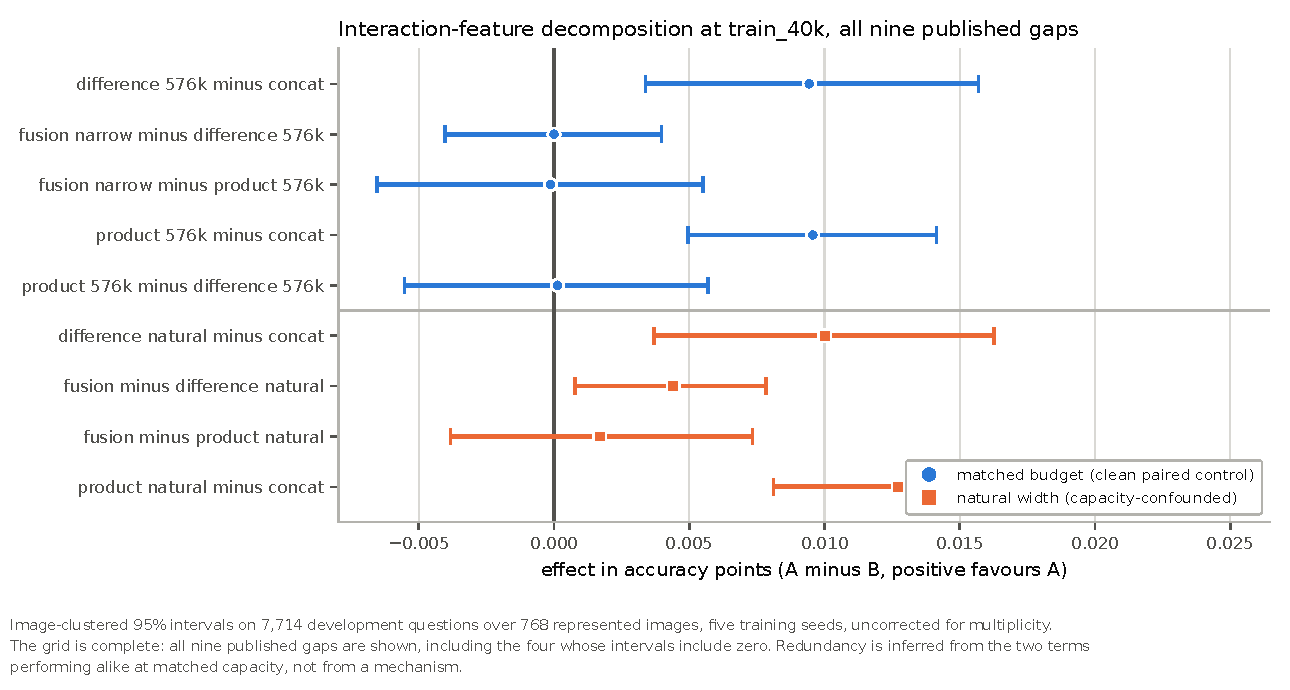
\includegraphics[width=\textwidth]{ve1/VE1-FIG-A1.pdf}
\caption[Interaction-feature decomposition at matched capacity.]{Interaction-feature decomposition at matched capacity. Either interaction term alone recovers most of the fusion gain at an equal parameter budget, and the two terms behave alike. Uncertainty: image-clustered 95 per cent evaluation-sampling intervals, clustered on the represented development imageId and conditioning on the fixed trained seed set. Nominal and uncorrected for multiplicity. Redundancy is inferred from the two terms performing alike at matched capacity, not from a mechanism. The natural-width contrasts are capacity-confounded. Development set, train\_40k, five training seeds. The grid is complete: all nine published gaps are shown, including the four whose intervals include zero.}
\label{fig:appA-interaction}
\end{figure}

\begin{figure}[p]
\centering
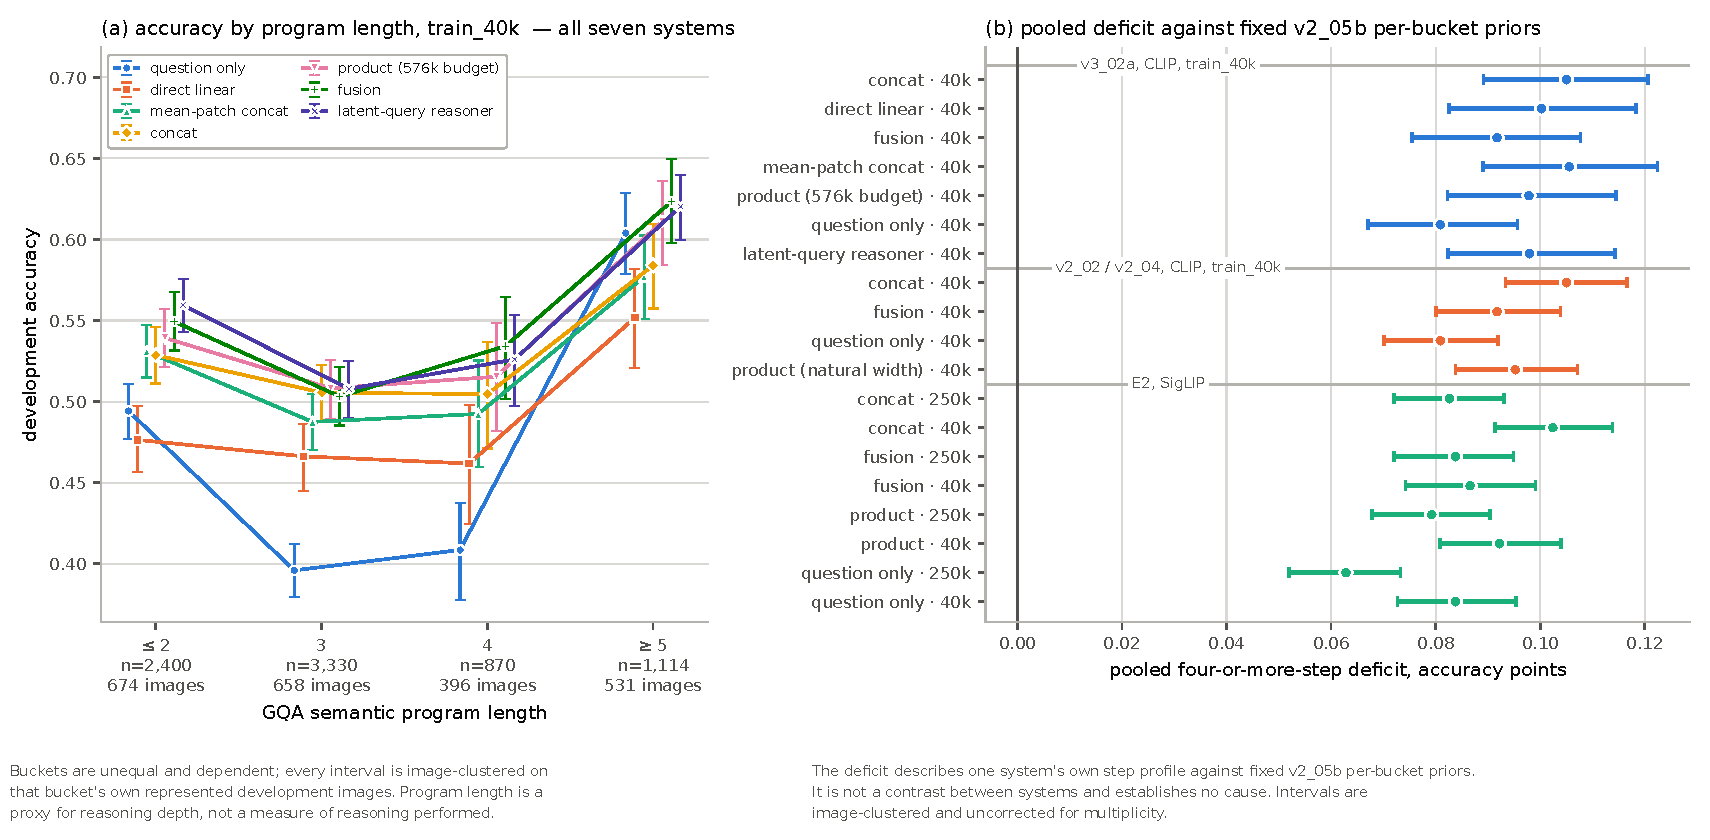
\includegraphics[width=\textwidth]{ve1/VE1-FIG-04-FULL.pdf}
\caption[Accuracy by program length, all systems.]{Accuracy by reasoning depth and the pooled four-or-more-step deficit. A pooled deficit at four or more reasoning steps persists across both frozen encoders, across training scales and across head families. Uncertainty: image-clustered 95 per cent evaluation-sampling intervals, clustered on the represented development imageId and conditioning on the fixed trained seed set. Nominal and uncorrected for multiplicity. The deficit is measured against fixed v2\_05b per-bucket priors and describes one system's step profile; it is not a contrast between systems and establishes no cause. Buckets are unequal and dependent, so every interval is clustered on the bucket's own represented development images; the per-bucket question and image counts must be printed. Step counts come from the GQA semantic program length, which is a proxy for reasoning depth, not a measure of reasoning.}
\label{fig:appA-depth-full}
\end{figure}

\begin{figure}[p]
\centering
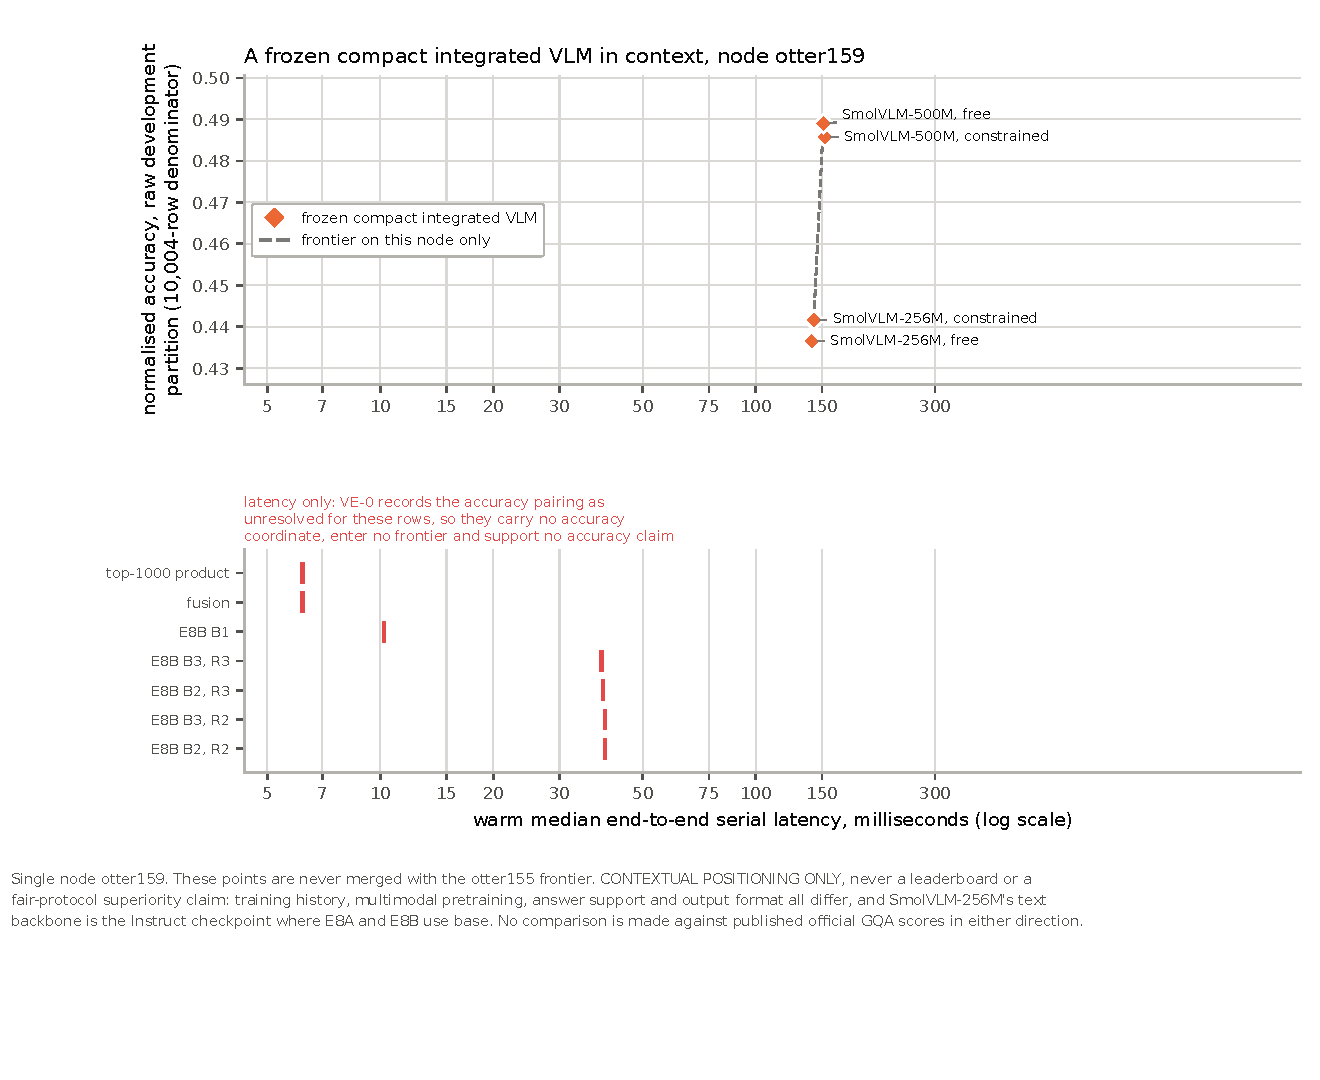
\includegraphics[width=\textwidth]{ve1/VE1-FIG-A5.pdf}
\caption[Compact VLM in context.]{Compact VLM in context. A frozen compact integrated VLM can be placed in context against these lightweight systems on one node. Uncertainty: none is drawn. Each latency is a warm median over repeated passes, not an estimate carrying sampling uncertainty. CONTEXTUAL POSITIONING ONLY, never a leaderboard or fair-protocol superiority claim. Training history, multimodal pretraining, answer support and output format all differ, and SmolVLM-256M's text backbone is the Instruct checkpoint where E8A and E8B use base. No comparison is made against published official GQA scores in either direction, because the split, the answer support and the scorer all differ. Single node otter159; these points are never merged with the otter155 frontier. Arm codes: A0p = CLIP question encoder; A1 = frozen pretrained SmolLM2-135M question encoder; B1 = lightweight classifier readout; B2 = random SmolLM2-135M readout; B3 = pretrained SmolLM2-135M readout; R2 = trie-constrained greedy generation; R3 = free greedy generation with a fixed token cap; reasoner = latent-query reasoner. `free' and `constrained' on a SmolVLM point are free greedy and answer-support-constrained generation.}
\label{fig:appA-e9}
\end{figure}

\clearpage
\begin{table}[p]
\centering
\caption[Training-scale effects, frozen-SLM families.]{Training-scale effects, frozen-SLM families. How much does labelled training scale move each SLM-interface system? Development-set result on one GQA subset. No held-out generalisation is claimed. Both pretraining-effect intervals contain zero and the seeds disagree in sign; they establish neither equivalence nor the absence of an effect. The 135M-to-360M step is whole-system capacity sensitivity, not an isolated causal language-model-size effect: trainable capacity moves too, 21,343,808 to 21,540,800 parameters, because the projection width follows the hidden size. An interval containing zero is an absence of a detected effect and establishes neither equivalence nor the absence of an effect. B3 at train\_40k has an across-training-seed sd of 0.02795 and must always be shown with its seed spread.}
\label{tab:appA-scale-effects}
\begingroup\scriptsize\setlength{\tabcolsep}{2pt}
\makeatletter
\let\appAArrayParboxRestore\@arrayparboxrestore
\def\@arrayparboxrestore{\appAArrayParboxRestore\raggedright\let\\\tabularnewline}
\makeatother
\renewcommand{\_}{\textunderscore\allowbreak}
\renewenvironment{longtable}[1]{\begin{tabular}{|p{0.13\textwidth}|p{0.17\textwidth}|p{0.11\textwidth}|p{0.15\textwidth}|p{0.07\textwidth}|p{0.11\textwidth}|p{0.17\textwidth}|}}{\end{tabular}}
\let\endhead\relax
% Generated by tools/tab2latex.py; do not edit.
% Presentation metadata: {"header_map":{"95% CI (image-clustered)":"95% CI (image-clustered)","effect (250k minus 40k)":"Effect (250k minus 40k)","evidence id":"Evidence id","excludes zero":"Excludes zero","language model":"Language model","sd (training seeds, ddof=1)":"SD (training seeds, ddof=1)","system":"System"},"source_headers":["system","language model","effect (250k minus 40k)","95% CI (image-clustered)","excludes zero","sd (training seeds, ddof=1)","evidence id"],"thousands":false}
\begin{longtable}{|l|l|l|l|l|l|l|}
\hline
System & Language model & Effect (250k minus 40k) & 95\% CI (image-clustered) & Excludes zero & SD (training seeds, ddof=1) & Evidence id \\ \hline
\endhead
B4 (answer side) & SmolLM2-360M, pretrained & 0.06771 & [0.05800, 0.07738] & true & 0.01208 & EV-CON-E10.scale\_effect\_B4 \\ \hline
B4r (answer side) & SmolLM2-360M, random & 0.06326 & [0.05287, 0.07296] & true & 0.00611 & EV-CON-E10.scale\_effect\_B4r \\ \hline
B1 (answer side (no language model)) & none (lightweight classifier readout) & 0.04887 & [0.03943, 0.05801] & true & not available & EV-CON-E8B.scale\_effect\_B1 \\ \hline
B2 (answer side) & SmolLM2-135M, random & 0.06693 & [0.05683, 0.07633] & true & not available & EV-CON-E8B.scale\_effect\_B2 \\ \hline
B3 (answer side) & SmolLM2-135M, pretrained & 0.08681 & [0.07781, 0.09640] & true & not available & EV-CON-E8B.scale\_effect\_B3 \\ \hline
\end{longtable}

\endgroup
\end{table}

\clearpage
\begin{table}[p]
\centering
\caption[Full slice statistics, v2\_02, 40k.]{Full slice statistics. What is every per-type, per-structure and per-step-bucket value, with its counts? Development-set result on one GQA subset. No held-out generalisation is claimed. E8A's projected interface is a learned common width, not a naturally shared pretrained embedding space. A1 minus A1r is the only clean within-size question-side pretraining contrast; A1 minus A0p also changes the representation space and the interface. Slices are unequal and dependent; every interval is clustered on the slice's own represented development images, never on rows. A drop under a wrong or removed image demonstrates reliance on the image. It is NOT proof of robust visual reasoning, of grounding or of compositional understanding. The question-only drop is exactly zero by construction and is a control, not a result. A system-level comparison. Input granularity, architecture and parameter count change together, so token-level access is not isolated as the cause. The step-bucket slices are printed as at most 2, at least 4 and at least 5 for the buckets $\leq$2, $\geq$4 and $\geq$5; the values are unchanged.}
\label{tab:appA-slices}
\begingroup\scriptsize\setlength{\tabcolsep}{2pt}
\makeatletter
\let\appAArrayParboxRestore\@arrayparboxrestore
\def\@arrayparboxrestore{\appAArrayParboxRestore\raggedright\let\\\tabularnewline}
\makeatother
\renewcommand{\_}{\textunderscore\allowbreak}
\renewenvironment{longtable}[1]{\begin{tabular}{|p{0.07\textwidth}|p{0.12\textwidth}|p{0.05\textwidth}|p{0.11\textwidth}|p{0.15\textwidth}|p{0.08\textwidth}|p{0.15\textwidth}|p{0.07\textwidth}|p{0.07\textwidth}|}}{\end{tabular}}
\let\endhead\relax
% Generated by tools/tab2latex.py; do not edit.
% Presentation metadata: {"columns":["family","system","scale","slice kind","slice","point estimate","95% CI (image-clustered)","n questions","n images"],"dropped_columns":["slice id","quantity","metric","counts provenance","evidence id"],"header_map":{"95% CI (image-clustered)":"95% CI (image-clustered)","family":"Family","n images":"n images","n questions":"n questions","point estimate":"Point estimate","scale":"Scale","slice":"Slice","slice kind":"Slice kind","system":"System"},"source_headers":["family","system","scale","slice kind","slice","point estimate","95% CI (image-clustered)","n questions","n images"],"thousands":true}
\begin{longtable}{|l|l|l|l|l|l|l|l|l|}
\hline
Family & System & Scale & Slice kind & Slice & Point estimate & 95\% CI (image-clustered) & n questions & n images \\ \hline
\endhead
v2\_02 & concat & 40k & semantic & semantic:attr & 0.46120 & [0.44560, 0.47637] & 2,964 & 691 \\ \hline
v2\_02 & concat & 40k & semantic & semantic:cat & 0.56583 & [0.50914, 0.61781] & 439 & 219 \\ \hline
v2\_02 & concat & 40k & semantic & semantic:global & 0.80736 & [0.75404, 0.85750] & 163 & 133 \\ \hline
v2\_02 & concat & 40k & semantic & semantic:obj & 0.59846 & [0.57540, 0.62234] & 1,170 & 547 \\ \hline
v2\_02 & concat & 40k & semantic & semantic:rel & 0.53553 & [0.51452, 0.55627] & 2,978 & 570 \\ \hline
v2\_02 & concat & 40k & program length & steps:3 & 0.50559 & [0.48805, 0.52312] & 3,330 & 658 \\ \hline
v2\_02 & concat & 40k & program length & steps:4 & 0.50460 & [0.47071, 0.53715] & 870 & 396 \\ \hline
v2\_02 & concat & 40k & program length & steps: at least 5 & 0.58402 & [0.55945, 0.60991] & 1,114 & 531 \\ \hline
v2\_02 & concat & 40k & program length & steps: at most 2 & 0.52867 & [0.51247, 0.54586] & 2,400 & 674 \\ \hline
v2\_02 & concat & 40k & structural & structural:choose & 0.57697 & [0.55182, 0.60113] & 1,042 & 465 \\ \hline
v2\_02 & concat & 40k & structural & structural:compare & 0.57881 & [0.53597, 0.62451] & 302 & 226 \\ \hline
v2\_02 & concat & 40k & structural & structural:logical & 0.57848 & [0.55481, 0.60342] & 1,236 & 561 \\ \hline
v2\_02 & concat & 40k & structural & structural:query & 0.47951 & [0.45676, 0.50277] & 3,104 & 687 \\ \hline
v2\_02 & concat & 40k & structural & structural:verify & 0.52345 & [0.50607, 0.54061] & 2,030 & 615 \\ \hline
v2\_02 & fusion & 40k & semantic & semantic:attr & 0.46444 & [0.44697, 0.48159] & 2,964 & 691 \\ \hline
v2\_02 & fusion & 40k & semantic & semantic:cat & 0.56355 & [0.51162, 0.61340] & 439 & 219 \\ \hline
v2\_02 & fusion & 40k & semantic & semantic:global & 0.80123 & [0.74267, 0.85522] & 163 & 133 \\ \hline
v2\_02 & fusion & 40k & semantic & semantic:obj & 0.64103 & [0.61682, 0.66633] & 1,170 & 547 \\ \hline
v2\_02 & fusion & 40k & semantic & semantic:rel & 0.55359 & [0.53251, 0.57507] & 2,978 & 570 \\ \hline
v2\_02 & fusion & 40k & program length & steps:3 & 0.50312 & [0.48459, 0.52153] & 3,330 & 658 \\ \hline
v2\_02 & fusion & 40k & program length & steps:4 & 0.53425 & [0.50284, 0.56727] & 870 & 396 \\ \hline
v2\_02 & fusion & 40k & program length & steps: at least 5 & 0.62334 & [0.59786, 0.64950] & 1,114 & 531 \\ \hline
v2\_02 & fusion & 40k & program length & steps: at most 2 & 0.54942 & [0.53239, 0.56697] & 2,400 & 674 \\ \hline
v2\_02 & fusion & 40k & structural & structural:choose & 0.55393 & [0.52733, 0.58099] & 1,042 & 465 \\ \hline
v2\_02 & fusion & 40k & structural & structural:compare & 0.55364 & [0.50779, 0.60206] & 302 & 226 \\ \hline
v2\_02 & fusion & 40k & structural & structural:logical & 0.61650 & [0.59179, 0.64201] & 1,236 & 561 \\ \hline
v2\_02 & fusion & 40k & structural & structural:query & 0.48015 & [0.45799, 0.50385] & 3,104 & 687 \\ \hline
v2\_02 & fusion & 40k & structural & structural:verify & 0.56966 & [0.55042, 0.58836] & 2,030 & 615 \\ \hline
\end{longtable}

\endgroup
\end{table}

\clearpage
\begin{table}[p]
\centering
\caption[Full slice statistics, v2\_05c, 40k.]{Full slice statistics, continued: v2\_05c, 40k. Same quantities, uncertainty notation and caveats as Table~\ref{tab:appA-slices}.}
\label{tab:appA-slices-v205c}
\begingroup\scriptsize\setlength{\tabcolsep}{2pt}
\makeatletter
\let\appAArrayParboxRestore\@arrayparboxrestore
\def\@arrayparboxrestore{\appAArrayParboxRestore\raggedright\let\\\tabularnewline}
\makeatother
\renewcommand{\_}{\textunderscore\allowbreak}
\renewenvironment{longtable}[1]{\begin{tabular}{|p{0.07\textwidth}|p{0.12\textwidth}|p{0.05\textwidth}|p{0.11\textwidth}|p{0.15\textwidth}|p{0.08\textwidth}|p{0.15\textwidth}|p{0.07\textwidth}|p{0.07\textwidth}|}}{\end{tabular}}
\let\endhead\relax
% Generated by tools/tab2latex.py; do not edit.
% Presentation metadata: {"columns":["family","system","scale","slice kind","slice","point estimate","95% CI (image-clustered)","n questions","n images"],"dropped_columns":["slice id","quantity","metric","counts provenance","evidence id"],"header_map":{"95% CI (image-clustered)":"95% CI (image-clustered)","family":"Family","n images":"n images","n questions":"n questions","point estimate":"Point estimate","scale":"Scale","slice":"Slice","slice kind":"Slice kind","system":"System"},"source_headers":["family","system","scale","slice kind","slice","point estimate","95% CI (image-clustered)","n questions","n images"],"thousands":true}
\begin{longtable}{|l|l|l|l|l|l|l|l|l|}
\hline
Family & System & Scale & Slice kind & Slice & Point estimate & 95\% CI (image-clustered) & n questions & n images \\ \hline
\endhead
v2\_05c & fusion minus concat & 40k & semantic & semantic:attr & 0.00324 & [-0.00762, 0.01441] & 2,964 & 691 \\ \hline
v2\_05c & fusion minus concat & 40k & semantic & semantic:attr & -0.00439 & [-0.02343, 0.01387] & 2,964 & 691 \\ \hline
v2\_05c & fusion minus concat & 40k & semantic & semantic:cat & -0.00228 & [-0.01639, 0.01264] & 439 & 219 \\ \hline
v2\_05c & fusion minus concat & 40k & semantic & semantic:cat & 0.00456 & [-0.02734, 0.03633] & 439 & 219 \\ \hline
v2\_05c & fusion minus concat & 40k & semantic & semantic:global & -0.00613 & [-0.03558, 0.02099] & 163 & 133 \\ \hline
v2\_05c & fusion minus concat & 40k & semantic & semantic:global & -0.01840 & [-0.06876, 0.03068] & 163 & 133 \\ \hline
v2\_05c & fusion minus concat & 40k & semantic & semantic:obj & 0.04257 & [0.02300, 0.06247] & 1,170 & 547 \\ \hline
v2\_05c & fusion minus concat & 40k & semantic & semantic:obj & 0.03932 & [0.01424, 0.06444] & 1,170 & 547 \\ \hline
v2\_05c & fusion minus concat & 40k & semantic & semantic:rel & 0.01806 & [0.00921, 0.02780] & 2,978 & 570 \\ \hline
v2\_05c & fusion minus concat & 40k & semantic & semantic:rel & 0.02552 & [0.01043, 0.04109] & 2,978 & 570 \\ \hline
v2\_05c & fusion minus concat & 40k & program length & steps:3 & -0.00246 & [-0.01163, 0.00644] & 3,330 & 658 \\ \hline
v2\_05c & fusion minus concat & 40k & program length & steps:3 & 0.00480 & [-0.00991, 0.01914] & 3,330 & 658 \\ \hline
v2\_05c & fusion minus concat & 40k & program length & steps:4 & 0.02966 & [0.00912, 0.05049] & 870 & 396 \\ \hline
v2\_05c & fusion minus concat & 40k & program length & steps:4 & 0.02644 & [-0.00117, 0.05474] & 870 & 396 \\ \hline
v2\_05c & fusion minus concat & 40k & program length & steps: at least 5 & 0.03932 & [0.01872, 0.05975] & 1,114 & 531 \\ \hline
v2\_05c & fusion minus concat & 40k & program length & steps: at least 5 & 0.03950 & [0.01297, 0.06595] & 1,114 & 531 \\ \hline
v2\_05c & fusion minus concat & 40k & program length & steps: at most 2 & 0.02075 & [0.00876, 0.03247] & 2,400 & 674 \\ \hline
v2\_05c & fusion minus concat & 40k & program length & steps: at most 2 & 0.01042 & [-0.00916, 0.03016] & 2,400 & 674 \\ \hline
v2\_05c & fusion minus concat & 40k & structural & structural:choose & -0.02303 & [-0.03669, -0.00954] & 1,042 & 465 \\ \hline
v2\_05c & fusion minus concat & 40k & structural & structural:choose & -0.01631 & [-0.03949, 0.00660] & 1,042 & 465 \\ \hline
v2\_05c & fusion minus concat & 40k & structural & structural:compare & -0.02517 & [-0.06598, 0.01355] & 302 & 226 \\ \hline
v2\_05c & fusion minus concat & 40k & structural & structural:compare & -0.04305 & [-0.10065, 0.01347] & 302 & 226 \\ \hline
v2\_05c & fusion minus concat & 40k & structural & structural:logical & 0.03802 & [0.01687, 0.05815] & 1,236 & 561 \\ \hline
v2\_05c & fusion minus concat & 40k & structural & structural:logical & 0.04045 & [0.01403, 0.06760] & 1,236 & 561 \\ \hline
v2\_05c & fusion minus concat & 40k & structural & structural:query & 0.00064 & [-0.00711, 0.00810] & 3,104 & 687 \\ \hline
v2\_05c & fusion minus concat & 40k & structural & structural:query & 0.00129 & [-0.01362, 0.01608] & 3,104 & 687 \\ \hline
v2\_05c & fusion minus concat & 40k & structural & structural:verify & 0.04621 & [0.03236, 0.06034] & 2,030 & 615 \\ \hline
v2\_05c & fusion minus concat & 40k & structural & structural:verify & 0.04138 & [0.02111, 0.06274] & 2,030 & 615 \\ \hline
\end{longtable}

\endgroup
\end{table}

\clearpage
\begin{table}[p]
\centering
\caption[Full slice statistics, v2\_06, 40k.]{Full slice statistics, continued: v2\_06, 40k. Same quantities, uncertainty notation and caveats as Table~\ref{tab:appA-slices}.}
\label{tab:appA-slices-v206}
\begingroup\scriptsize\setlength{\tabcolsep}{2pt}
\makeatletter
\let\appAArrayParboxRestore\@arrayparboxrestore
\def\@arrayparboxrestore{\appAArrayParboxRestore\raggedright\let\\\tabularnewline}
\makeatother
\renewcommand{\_}{\textunderscore\allowbreak}
\renewenvironment{longtable}[1]{\begin{tabular}{|p{0.07\textwidth}|p{0.12\textwidth}|p{0.05\textwidth}|p{0.11\textwidth}|p{0.15\textwidth}|p{0.08\textwidth}|p{0.15\textwidth}|p{0.07\textwidth}|p{0.07\textwidth}|}}{\end{tabular}}
\let\endhead\relax
% Generated by tools/tab2latex.py; do not edit.
% Presentation metadata: {"columns":["family","system","scale","slice kind","slice","quantity","point estimate","95% CI (image-clustered)","n questions","n images"],"dropped_columns":["slice id","metric","counts provenance","evidence id"],"header_map":{"95% CI (image-clustered)":"95% CI (image-clustered)","family":"Family","n images":"n images","n questions":"n questions","point estimate":"Point estimate","quantity":"Quantity","scale":"Scale","slice":"Slice","slice kind":"Slice kind","system":"System"},"source_headers":["family","system","scale","slice kind","slice","quantity","point estimate","95% CI (image-clustered)","n questions","n images"],"thousands":true}
\begin{longtable}{|l|l|l|l|l|l|l|l|l|l|}
\hline
Family & System & Scale & Slice kind & Slice & Quantity & Point estimate & 95\% CI (image-clustered) & n questions & n images \\ \hline
\endhead
v2\_06 & concat & 40k & structural & structural:choose & drop\_shuffled on the structural slice choose & 0.11536 & [0.08367, 0.14685] & 1,042 & 465 \\ \hline
v2\_06 & concat & 40k & structural & structural:choose & drop\_zeroed on the structural slice choose & 0.07351 & [0.04616, 0.10112] & 1,042 & 465 \\ \hline
v2\_06 & concat & 40k & structural & structural:compare & drop\_shuffled on the structural slice compare & 0.01060 & [-0.03542, 0.05856] & 302 & 226 \\ \hline
v2\_06 & concat & 40k & structural & structural:compare & drop\_zeroed on the structural slice compare & 0.02318 & [-0.01534, 0.06195] & 302 & 226 \\ \hline
v2\_06 & concat & 40k & structural & structural:logical & drop\_shuffled on the structural slice logical & 0.03366 & [0.00858, 0.06013] & 1,236 & 561 \\ \hline
v2\_06 & concat & 40k & structural & structural:logical & drop\_zeroed on the structural slice logical & 0.01796 & [-0.00245, 0.03945] & 1,236 & 561 \\ \hline
v2\_06 & concat & 40k & structural & structural:query & drop\_shuffled on the structural slice query & 0.22610 & [0.20096, 0.25104] & 3,104 & 687 \\ \hline
v2\_06 & concat & 40k & structural & structural:query & drop\_zeroed on the structural slice query & 0.18428 & [0.16038, 0.20926] & 3,104 & 687 \\ \hline
v2\_06 & concat & 40k & structural & structural:verify & drop\_shuffled on the structural slice verify & 0.01793 & [-0.00046, 0.03533] & 2,030 & 615 \\ \hline
v2\_06 & concat & 40k & structural & structural:verify & drop\_zeroed on the structural slice verify & 0.04562 & [0.02907, 0.06133] & 2,030 & 615 \\ \hline
v2\_06 & fusion & 40k & structural & structural:choose & drop\_shuffled on the structural slice choose & 0.11344 & [0.08083, 0.14787] & 1,042 & 465 \\ \hline
v2\_06 & fusion & 40k & structural & structural:choose & drop\_zeroed on the structural slice choose & 0.05547 & [0.02595, 0.08566] & 1,042 & 465 \\ \hline
v2\_06 & fusion & 40k & structural & structural:compare & drop\_shuffled on the structural slice compare & 0.00861 & [-0.04576, 0.06736] & 302 & 226 \\ \hline
v2\_06 & fusion & 40k & structural & structural:compare & drop\_zeroed on the structural slice compare & -0.01854 & [-0.07774, 0.03988] & 302 & 226 \\ \hline
v2\_06 & fusion & 40k & structural & structural:logical & drop\_shuffled on the structural slice logical & 0.10275 & [0.06784, 0.13830] & 1,236 & 561 \\ \hline
v2\_06 & fusion & 40k & structural & structural:logical & drop\_zeroed on the structural slice logical & 0.06100 & [0.02810, 0.09203] & 1,236 & 561 \\ \hline
v2\_06 & fusion & 40k & structural & structural:query & drop\_shuffled on the structural slice query & 0.22674 & [0.20295, 0.25199] & 3,104 & 687 \\ \hline
v2\_06 & fusion & 40k & structural & structural:query & drop\_zeroed on the structural slice query & 0.18789 & [0.16325, 0.21355] & 3,104 & 687 \\ \hline
v2\_06 & fusion & 40k & structural & structural:verify & drop\_shuffled on the structural slice verify & 0.07350 & [0.04781, 0.10077] & 2,030 & 615 \\ \hline
v2\_06 & fusion & 40k & structural & structural:verify & drop\_zeroed on the structural slice verify & 0.10128 & [0.07835, 0.12445] & 2,030 & 615 \\ \hline
\end{longtable}

\endgroup
\end{table}

\clearpage
\begin{table}[p]
\centering
\caption[Full slice statistics, v3\_02a, 40k, part 1.]{Full slice statistics, continued: v3\_02a, 40k, systems part 1. Same quantities, uncertainty notation and caveats as Table~\ref{tab:appA-slices}.}
\label{tab:appA-slices-v302a-1}
\begingroup\scriptsize\setlength{\tabcolsep}{2pt}
\makeatletter
\let\appAArrayParboxRestore\@arrayparboxrestore
\def\@arrayparboxrestore{\appAArrayParboxRestore\raggedright\let\\\tabularnewline}
\makeatother
\renewcommand{\_}{\textunderscore\allowbreak}
\renewenvironment{longtable}[1]{\begin{tabular}{|p{0.07\textwidth}|p{0.12\textwidth}|p{0.05\textwidth}|p{0.11\textwidth}|p{0.15\textwidth}|p{0.08\textwidth}|p{0.15\textwidth}|p{0.07\textwidth}|p{0.07\textwidth}|}}{\end{tabular}}
\let\endhead\relax
% Generated by tools/tab2latex.py; do not edit.
% Presentation metadata: {"columns":["family","system","scale","slice kind","slice","quantity","point estimate","95% CI (image-clustered)","n questions","n images"],"dropped_columns":["slice id","metric","counts provenance","evidence id"],"header_map":{"95% CI (image-clustered)":"95% CI (image-clustered)","family":"Family","n images":"n images","n questions":"n questions","point estimate":"Point estimate","quantity":"Quantity","scale":"Scale","slice":"Slice","slice kind":"Slice kind","system":"System"},"source_headers":["family","system","scale","slice kind","slice","quantity","point estimate","95% CI (image-clustered)","n questions","n images"],"thousands":true}
\begin{longtable}{|l|l|l|l|l|l|l|l|l|l|}
\hline
Family & System & Scale & Slice kind & Slice & Quantity & Point estimate & 95\% CI (image-clustered) & n questions & n images \\ \hline
\endhead
v3\_02a & concat & 40k & program length & steps:3 & accuracy on the steps slice 3 & 0.50559 & [0.48758, 0.52263] & 3,330 & 658 \\ \hline
v3\_02a & concat & 40k & program length & steps:4 & accuracy on the steps slice 4 & 0.50460 & [0.47113, 0.53689] & 870 & 396 \\ \hline
v3\_02a & concat & 40k & program length & steps: at least 4 & pooled at-least-4-step deficit on the steps slice at least 4 (combined) & 0.10502 & [0.08915, 0.12065] & 1,984 & not available \\ \hline
v3\_02a & concat & 40k & program length & steps: at least 5 & accuracy on the steps slice at least 5 & 0.58402 & [0.55744, 0.60933] & 1,114 & 531 \\ \hline
v3\_02a & concat & 40k & program length & steps: at most 2 & accuracy on the steps slice at most 2 & 0.52867 & [0.51115, 0.54615] & 2,400 & 674 \\ \hline
v3\_02a & direct\_linear & 40k & program length & steps:3 & accuracy on the steps slice 3 & 0.46625 & [0.44511, 0.48610] & 3,330 & 658 \\ \hline
v3\_02a & direct\_linear & 40k & program length & steps:4 & accuracy on the steps slice 4 & 0.46184 & [0.42448, 0.49805] & 870 & 396 \\ \hline
v3\_02a & direct\_linear & 40k & program length & steps: at least 4 & pooled at-least-4-step deficit on the steps slice at least 4 (combined) & 0.10025 & [0.08254, 0.11827] & 1,984 & not available \\ \hline
v3\_02a & direct\_linear & 40k & program length & steps: at least 5 & accuracy on the steps slice at least 5 & 0.55171 & [0.52055, 0.58200] & 1,114 & 531 \\ \hline
v3\_02a & direct\_linear & 40k & program length & steps: at most 2 & accuracy on the steps slice at most 2 & 0.47642 & [0.45657, 0.49737] & 2,400 & 674 \\ \hline
v3\_02a & meanpatch\_concat & 40k & program length & steps:3 & accuracy on the steps slice 3 & 0.48751 & [0.47040, 0.50450] & 3,330 & 658 \\ \hline
v3\_02a & meanpatch\_concat & 40k & program length & steps:4 & accuracy on the steps slice 4 & 0.49241 & [0.45956, 0.52534] & 870 & 396 \\ \hline
v3\_02a & meanpatch\_concat & 40k & program length & steps: at least 4 & pooled at-least-4-step deficit on the steps slice at least 4 (combined) & 0.10554 & [0.08901, 0.12247] & 1,984 & not available \\ \hline
v3\_02a & meanpatch\_concat & 40k & program length & steps: at least 5 & accuracy on the steps slice at least 5 & 0.57702 & [0.55113, 0.60240] & 1,114 & 531 \\ \hline
v3\_02a & meanpatch\_concat & 40k & program length & steps: at most 2 & accuracy on the steps slice at most 2 & 0.53092 & [0.51484, 0.54732] & 2,400 & 674 \\ \hline
v3\_02a & question\_only & 40k & program length & steps:3 & accuracy on the steps slice 3 & 0.39592 & [0.37970, 0.41225] & 3,330 & 658 \\ \hline
v3\_02a & question\_only & 40k & program length & steps:4 & accuracy on the steps slice 4 & 0.40851 & [0.37775, 0.43747] & 870 & 396 \\ \hline
v3\_02a & question\_only & 40k & program length & steps: at least 4 & pooled at-least-4-step deficit on the steps slice at least 4 (combined) & 0.08090 & [0.06710, 0.09561] & 1,984 & not available \\ \hline
v3\_02a & question\_only & 40k & program length & steps: at least 5 & accuracy on the steps slice at least 5 & 0.60395 & [0.57851, 0.62886] & 1,114 & 531 \\ \hline
v3\_02a & question\_only & 40k & program length & steps: at most 2 & accuracy on the steps slice at most 2 & 0.49425 & [0.47688, 0.51065] & 2,400 & 674 \\ \hline
\end{longtable}

\endgroup
\end{table}

\clearpage
\begin{table}[p]
\centering
\caption[Full slice statistics, v3\_02a, 40k, part 2.]{Full slice statistics, continued: v3\_02a, 40k, systems part 2. Same quantities, uncertainty notation and caveats as Table~\ref{tab:appA-slices}.}
\label{tab:appA-slices-v302a-2}
\begingroup\scriptsize\setlength{\tabcolsep}{2pt}
\makeatletter
\let\appAArrayParboxRestore\@arrayparboxrestore
\def\@arrayparboxrestore{\appAArrayParboxRestore\raggedright\let\\\tabularnewline}
\makeatother
\renewcommand{\_}{\textunderscore\allowbreak}
\renewenvironment{longtable}[1]{\begin{tabular}{|p{0.07\textwidth}|p{0.12\textwidth}|p{0.05\textwidth}|p{0.11\textwidth}|p{0.15\textwidth}|p{0.08\textwidth}|p{0.15\textwidth}|p{0.07\textwidth}|p{0.07\textwidth}|}}{\end{tabular}}
\let\endhead\relax
% Generated by tools/tab2latex.py; do not edit.
% Presentation metadata: {"columns":["family","system","scale","slice kind","slice","point estimate","95% CI (image-clustered)","n questions","n images"],"dropped_columns":["slice id","quantity","metric","counts provenance","evidence id"],"header_map":{"95% CI (image-clustered)":"95% CI (image-clustered)","family":"Family","n images":"n images","n questions":"n questions","point estimate":"Point estimate","scale":"Scale","slice":"Slice","slice kind":"Slice kind","system":"System"},"source_headers":["family","system","scale","slice kind","slice","point estimate","95% CI (image-clustered)","n questions","n images"],"thousands":true}
\begin{longtable}{|l|l|l|l|l|l|l|l|l|}
\hline
Family & System & Scale & Slice kind & Slice & Point estimate & 95\% CI (image-clustered) & n questions & n images \\ \hline
\endhead
v3\_02a & fusion & 40k & program length & steps:3 & 0.50312 & [0.48522, 0.52139] & 3,330 & 658 \\ \hline
v3\_02a & fusion & 40k & program length & steps:4 & 0.53425 & [0.50177, 0.56433] & 870 & 396 \\ \hline
v3\_02a & fusion & 40k & program length & steps: at least 4 & 0.09175 & [0.07548, 0.10771] & 1,984 & not available \\ \hline
v3\_02a & fusion & 40k & program length & steps: at least 5 & 0.62334 & [0.59772, 0.64960] & 1,114 & 531 \\ \hline
v3\_02a & fusion & 40k & program length & steps: at most 2 & 0.54942 & [0.53147, 0.56744] & 2,400 & 674 \\ \hline
v3\_02a & product\_576k & 40k & program length & steps:3 & 0.50823 & [0.48935, 0.52559] & 3,330 & 658 \\ \hline
v3\_02a & product\_576k & 40k & program length & steps:4 & 0.51540 & [0.48182, 0.54868] & 870 & 396 \\ \hline
v3\_02a & product\_576k & 40k & program length & steps: at least 4 & 0.09784 & [0.08230, 0.11449] & 1,984 & not available \\ \hline
v3\_02a & product\_576k & 40k & program length & steps: at least 5 & 0.61113 & [0.58418, 0.63618] & 1,114 & 531 \\ \hline
v3\_02a & product\_576k & 40k & program length & steps: at most 2 & 0.53925 & [0.52139, 0.55702] & 2,400 & 674 \\ \hline
v3\_02a & reasoner & 40k & program length & steps:3 & 0.50791 & [0.48967, 0.52502] & 3,330 & 658 \\ \hline
v3\_02a & reasoner & 40k & program length & steps:4 & 0.52605 & [0.49718, 0.55341] & 870 & 396 \\ \hline
v3\_02a & reasoner & 40k & program length & steps: at least 4 & 0.09795 & [0.08236, 0.11434] & 1,984 & not available \\ \hline
v3\_02a & reasoner & 40k & program length & steps: at least 5 & 0.62029 & [0.59971, 0.63998] & 1,114 & 531 \\ \hline
v3\_02a & reasoner & 40k & program length & steps: at most 2 & 0.55944 & [0.54307, 0.57576] & 2,400 & 674 \\ \hline
\end{longtable}

\endgroup
\end{table}

\clearpage
\begin{table}[p]
\centering
\caption[Full slice statistics, E8A, 40k, semantic and program-length slices.]{Full slice statistics, continued: E8A, 40k, semantic and program-length slices. Same quantities, uncertainty notation and caveats as Table~\ref{tab:appA-slices}.}
\label{tab:appA-slices-e8a-40k-a}
\begingroup\scriptsize\setlength{\tabcolsep}{2pt}
\makeatletter
\let\appAArrayParboxRestore\@arrayparboxrestore
\def\@arrayparboxrestore{\appAArrayParboxRestore\raggedright\let\\\tabularnewline}
\makeatother
\renewcommand{\_}{\textunderscore\allowbreak}
\renewenvironment{longtable}[1]{\begin{tabular}{|p{0.07\textwidth}|p{0.12\textwidth}|p{0.05\textwidth}|p{0.11\textwidth}|p{0.15\textwidth}|p{0.08\textwidth}|p{0.15\textwidth}|p{0.07\textwidth}|p{0.07\textwidth}|}}{\end{tabular}}
\let\endhead\relax
% Generated by tools/tab2latex.py; do not edit.
% Presentation metadata: {"columns":["family","system","scale","slice kind","slice","point estimate","95% CI (image-clustered)","n questions","n images"],"dropped_columns":["slice id","quantity","metric","counts provenance","evidence id"],"header_map":{"95% CI (image-clustered)":"95% CI (image-clustered)","family":"Family","n images":"n images","n questions":"n questions","point estimate":"Point estimate","scale":"Scale","slice":"Slice","slice kind":"Slice kind","system":"System"},"source_headers":["family","system","scale","slice kind","slice","point estimate","95% CI (image-clustered)","n questions","n images"],"thousands":true}
\begin{longtable}{|l|l|l|l|l|l|l|l|l|}
\hline
Family & System & Scale & Slice kind & Slice & Point estimate & 95\% CI (image-clustered) & n questions & n images \\ \hline
\endhead
E8A & A0p & 40k & semantic & semantic:attr & 0.48201 & [0.46877, 0.49600] & 2,964 & 691 \\ \hline
E8A & A0p & 40k & semantic & semantic:cat & 0.58466 & [0.53364, 0.63377] & 439 & 219 \\ \hline
E8A & A0p & 40k & semantic & semantic:global & 0.81595 & [0.76534, 0.86670] & 163 & 133 \\ \hline
E8A & A0p & 40k & semantic & semantic:obj & 0.62194 & [0.60143, 0.64301] & 1,170 & 547 \\ \hline
E8A & A0p & 40k & semantic & semantic:rel & 0.54500 & [0.52537, 0.56501] & 2,978 & 570 \\ \hline
E8A & A0p & 40k & program length & steps:3 & 0.50731 & [0.49094, 0.52392] & 3,330 & 658 \\ \hline
E8A & A0p & 40k & program length & steps:4 & 0.53295 & [0.50381, 0.56314] & 870 & 396 \\ \hline
E8A & A0p & 40k & program length & steps: at least 5 & 0.62208 & [0.60188, 0.64383] & 1,114 & 531 \\ \hline
E8A & A0p & 40k & program length & steps: at most 2 & 0.55125 & [0.53467, 0.56767] & 2,400 & 674 \\ \hline
E8A & A1 & 40k & semantic & semantic:attr & 0.48032 & [0.46625, 0.49449] & 2,964 & 691 \\ \hline
E8A & A1 & 40k & semantic & semantic:cat & 0.58162 & [0.53218, 0.63017] & 439 & 219 \\ \hline
E8A & A1 & 40k & semantic & semantic:global & 0.73824 & [0.68888, 0.78788] & 163 & 133 \\ \hline
E8A & A1 & 40k & semantic & semantic:obj & 0.57151 & [0.55063, 0.59325] & 1,170 & 547 \\ \hline
E8A & A1 & 40k & semantic & semantic:rel & 0.54052 & [0.52044, 0.56073] & 2,978 & 570 \\ \hline
E8A & A1 & 40k & program length & steps:3 & 0.50110 & [0.48417, 0.51797] & 3,330 & 658 \\ \hline
E8A & A1 & 40k & program length & steps:4 & 0.53716 & [0.50736, 0.56636] & 870 & 396 \\ \hline
E8A & A1 & 40k & program length & steps: at least 5 & 0.57032 & [0.54841, 0.59131] & 1,114 & 531 \\ \hline
E8A & A1 & 40k & program length & steps: at most 2 & 0.54431 & [0.52861, 0.55941] & 2,400 & 674 \\ \hline
E8A & A1r & 40k & semantic & semantic:attr & 0.42735 & [0.41473, 0.44072] & 2,964 & 691 \\ \hline
E8A & A1r & 40k & semantic & semantic:cat & 0.51329 & [0.46008, 0.56375] & 439 & 219 \\ \hline
E8A & A1r & 40k & semantic & semantic:global & 0.75665 & [0.70614, 0.80503] & 163 & 133 \\ \hline
E8A & A1r & 40k & semantic & semantic:obj & 0.55043 & [0.52998, 0.57175] & 1,170 & 547 \\ \hline
E8A & A1r & 40k & semantic & semantic:rel & 0.51164 & [0.49322, 0.53070] & 2,978 & 570 \\ \hline
E8A & A1r & 40k & program length & steps:3 & 0.46026 & [0.44394, 0.47657] & 3,330 & 658 \\ \hline
E8A & A1r & 40k & program length & steps:4 & 0.50766 & [0.47792, 0.53586] & 870 & 396 \\ \hline
E8A & A1r & 40k & program length & steps: at least 5 & 0.54488 & [0.52363, 0.56579] & 1,114 & 531 \\ \hline
E8A & A1r & 40k & program length & steps: at most 2 & 0.50069 & [0.48634, 0.51615] & 2,400 & 674 \\ \hline
\end{longtable}

\endgroup
\end{table}

\clearpage
\begin{table}[p]
\centering
\caption[Full slice statistics, E8A, 40k, structural slices.]{Full slice statistics, continued: E8A, 40k, structural slices. Same quantities, uncertainty notation and caveats as Table~\ref{tab:appA-slices}.}
\label{tab:appA-slices-e8a-40k-b}
\begingroup\scriptsize\setlength{\tabcolsep}{2pt}
\makeatletter
\let\appAArrayParboxRestore\@arrayparboxrestore
\def\@arrayparboxrestore{\appAArrayParboxRestore\raggedright\let\\\tabularnewline}
\makeatother
\renewcommand{\_}{\textunderscore\allowbreak}
\renewenvironment{longtable}[1]{\begin{tabular}{|p{0.07\textwidth}|p{0.12\textwidth}|p{0.05\textwidth}|p{0.11\textwidth}|p{0.15\textwidth}|p{0.08\textwidth}|p{0.15\textwidth}|p{0.07\textwidth}|p{0.07\textwidth}|}}{\end{tabular}}
\let\endhead\relax
% Generated by tools/tab2latex.py; do not edit.
% Presentation metadata: {"columns":["family","system","scale","slice kind","slice","quantity","point estimate","95% CI (image-clustered)","n questions","n images"],"dropped_columns":["slice id","metric","counts provenance","evidence id"],"header_map":{"95% CI (image-clustered)":"95% CI (image-clustered)","family":"Family","n images":"n images","n questions":"n questions","point estimate":"Point estimate","quantity":"Quantity","scale":"Scale","slice":"Slice","slice kind":"Slice kind","system":"System"},"source_headers":["family","system","scale","slice kind","slice","quantity","point estimate","95% CI (image-clustered)","n questions","n images"],"thousands":true}
\begin{longtable}{|l|l|l|l|l|l|l|l|l|l|}
\hline
Family & System & Scale & Slice kind & Slice & Quantity & Point estimate & 95\% CI (image-clustered) & n questions & n images \\ \hline
\endhead
E8A & A0p & 40k & structural & structural:choose & accuracy on the structural slice choose & 0.62572 & [0.60375, 0.64822] & 1,042 & 465 \\ \hline
E8A & A0p & 40k & structural & structural:compare & accuracy on the structural slice compare & 0.60375 & [0.56250, 0.64422] & 302 & 226 \\ \hline
E8A & A0p & 40k & structural & structural:logical & accuracy on the structural slice logical & 0.60518 & [0.58479, 0.62612] & 1,236 & 561 \\ \hline
E8A & A0p & 40k & structural & structural:query & accuracy on the structural slice query & 0.47541 & [0.45461, 0.49810] & 3,104 & 687 \\ \hline
E8A & A0p & 40k & structural & structural:verify & accuracy on the structural slice verify & 0.54729 & [0.53109, 0.56323] & 2,030 & 615 \\ \hline
E8A & A1 & 40k & structural & structural:choose & accuracy on the structural slice choose & 0.60781 & [0.58279, 0.63309] & 1,042 & 465 \\ \hline
E8A & A1 & 40k & structural & structural:compare & accuracy on the structural slice compare & 0.60927 & [0.56902, 0.64955] & 302 & 226 \\ \hline
E8A & A1 & 40k & structural & structural:logical & accuracy on the structural slice logical & 0.56499 & [0.54507, 0.58542] & 1,236 & 561 \\ \hline
E8A & A1 & 40k & structural & structural:query & accuracy on the structural slice query & 0.47025 & [0.44792, 0.49339] & 3,104 & 687 \\ \hline
E8A & A1 & 40k & structural & structural:verify & accuracy on the structural slice verify & 0.54302 & [0.52558, 0.55872] & 2,030 & 615 \\ \hline
E8A & A1r & 40k & structural & structural:choose & accuracy on the structural slice choose & 0.48305 & [0.45862, 0.50734] & 1,042 & 465 \\ \hline
E8A & A1r & 40k & structural & structural:compare & accuracy on the structural slice compare & 0.58278 & [0.54637, 0.61939] & 302 & 226 \\ \hline
E8A & A1r & 40k & structural & structural:logical & accuracy on the structural slice logical & 0.53910 & [0.51933, 0.55869] & 1,236 & 561 \\ \hline
E8A & A1r & 40k & structural & structural:query & accuracy on the structural slice query & 0.44384 & [0.42288, 0.46370] & 3,104 & 687 \\ \hline
E8A & A1r & 40k & structural & structural:verify & accuracy on the structural slice verify & 0.52200 & [0.50748, 0.53561] & 2,030 & 615 \\ \hline
\end{longtable}

\endgroup
\end{table}

\clearpage
\begin{table}[p]
\centering
\caption[Full slice statistics, E8A, 250k, semantic and program-length slices.]{Full slice statistics, continued: E8A, 250k, semantic and program-length slices. Same quantities, uncertainty notation and caveats as Table~\ref{tab:appA-slices}.}
\label{tab:appA-slices-e8a-250k-a}
\begingroup\scriptsize\setlength{\tabcolsep}{2pt}
\makeatletter
\let\appAArrayParboxRestore\@arrayparboxrestore
\def\@arrayparboxrestore{\appAArrayParboxRestore\raggedright\let\\\tabularnewline}
\makeatother
\renewcommand{\_}{\textunderscore\allowbreak}
\renewenvironment{longtable}[1]{\begin{tabular}{|p{0.07\textwidth}|p{0.12\textwidth}|p{0.05\textwidth}|p{0.11\textwidth}|p{0.15\textwidth}|p{0.08\textwidth}|p{0.15\textwidth}|p{0.07\textwidth}|p{0.07\textwidth}|}}{\end{tabular}}
\let\endhead\relax
% Generated by tools/tab2latex.py; do not edit.
% Presentation metadata: {"columns":["family","system","scale","slice kind","slice","quantity","point estimate","95% CI (image-clustered)","n questions","n images"],"dropped_columns":["slice id","metric","counts provenance","evidence id"],"header_map":{"95% CI (image-clustered)":"95% CI (image-clustered)","family":"Family","n images":"n images","n questions":"n questions","point estimate":"Point estimate","quantity":"Quantity","scale":"Scale","slice":"Slice","slice kind":"Slice kind","system":"System"},"source_headers":["family","system","scale","slice kind","slice","quantity","point estimate","95% CI (image-clustered)","n questions","n images"],"thousands":true}
\begin{longtable}{|l|l|l|l|l|l|l|l|l|l|}
\hline
Family & System & Scale & Slice kind & Slice & Quantity & Point estimate & 95\% CI (image-clustered) & n questions & n images \\ \hline
\endhead
E8A & A0p & 250k & semantic & semantic:attr & accuracy on the semantic slice attr & 0.51395 & [0.50017, 0.52779] & 2,964 & 691 \\ \hline
E8A & A0p & 250k & semantic & semantic:cat & accuracy on the semantic slice cat & 0.63857 & [0.58923, 0.68417] & 439 & 219 \\ \hline
E8A & A0p & 250k & semantic & semantic:global & accuracy on the semantic slice global & 0.85890 & [0.81045, 0.90389] & 163 & 133 \\ \hline
E8A & A0p & 250k & semantic & semantic:obj & accuracy on the semantic slice obj & 0.72108 & [0.70117, 0.74087] & 1,170 & 547 \\ \hline
E8A & A0p & 250k & semantic & semantic:rel & accuracy on the semantic slice rel & 0.60387 & [0.58426, 0.62269] & 2,978 & 570 \\ \hline
E8A & A0p & 250k & program length & steps:3 & accuracy on the steps slice 3 & 0.55536 & [0.53992, 0.57135] & 3,330 & 658 \\ \hline
E8A & A0p & 250k & program length & steps:4 & accuracy on the steps slice 4 & 0.57280 & [0.54215, 0.60215] & 870 & 396 \\ \hline
E8A & A0p & 250k & program length & steps: at least 5 & accuracy on the steps slice at least 5 & 0.71424 & [0.69256, 0.73580] & 1,114 & 531 \\ \hline
E8A & A0p & 250k & program length & steps: at most 2 & accuracy on the steps slice at most 2 & 0.60097 & [0.58492, 0.61661] & 2,400 & 674 \\ \hline
E8A & A1 & 250k & semantic & semantic:attr & accuracy on the semantic slice attr & 0.50124 & [0.48818, 0.51424] & 2,964 & 691 \\ \hline
E8A & A1 & 250k & semantic & semantic:cat & accuracy on the semantic slice cat & 0.61731 & [0.56674, 0.66594] & 439 & 219 \\ \hline
E8A & A1 & 250k & semantic & semantic:global & accuracy on the semantic slice global & 0.86094 & [0.81687, 0.90357] & 163 & 133 \\ \hline
E8A & A1 & 250k & semantic & semantic:obj & accuracy on the semantic slice obj & 0.67920 & [0.65826, 0.69989] & 1,170 & 547 \\ \hline
E8A & A1 & 250k & semantic & semantic:rel & accuracy on the semantic slice rel & 0.58081 & [0.56113, 0.59975] & 2,978 & 570 \\ \hline
E8A & A1 & 250k & program length & steps:3 & accuracy on the steps slice 3 & 0.53383 & [0.51646, 0.55140] & 3,330 & 658 \\ \hline
E8A & A1 & 250k & program length & steps:4 & accuracy on the steps slice 4 & 0.55057 & [0.52130, 0.58095] & 870 & 396 \\ \hline
E8A & A1 & 250k & program length & steps: at least 5 & accuracy on the steps slice at least 5 & 0.67923 & [0.65904, 0.70012] & 1,114 & 531 \\ \hline
E8A & A1 & 250k & program length & steps: at most 2 & accuracy on the steps slice at most 2 & 0.58667 & [0.57193, 0.60214] & 2,400 & 674 \\ \hline
E8A & A1r & 250k & semantic & semantic:attr & accuracy on the semantic slice attr & 0.45502 & [0.44004, 0.46978] & 2,964 & 691 \\ \hline
E8A & A1r & 250k & semantic & semantic:cat & accuracy on the semantic slice cat & 0.58238 & [0.52739, 0.63471] & 439 & 219 \\ \hline
E8A & A1r & 250k & semantic & semantic:global & accuracy on the semantic slice global & 0.81800 & [0.76483, 0.87026] & 163 & 133 \\ \hline
E8A & A1r & 250k & semantic & semantic:obj & accuracy on the semantic slice obj & 0.56439 & [0.54320, 0.58565] & 1,170 & 547 \\ \hline
E8A & A1r & 250k & semantic & semantic:rel & accuracy on the semantic slice rel & 0.55418 & [0.53444, 0.57452] & 2,978 & 570 \\ \hline
E8A & A1r & 250k & program length & steps:3 & accuracy on the steps slice 3 & 0.49720 & [0.47966, 0.51452] & 3,330 & 658 \\ \hline
E8A & A1r & 250k & program length & steps:4 & accuracy on the steps slice 4 & 0.53142 & [0.50284, 0.56164] & 870 & 396 \\ \hline
E8A & A1r & 250k & program length & steps: at least 5 & accuracy on the steps slice at least 5 & 0.56014 & [0.53820, 0.58441] & 1,114 & 531 \\ \hline
E8A & A1r & 250k & program length & steps: at most 2 & accuracy on the steps slice at most 2 & 0.54431 & [0.52815, 0.56141] & 2,400 & 674 \\ \hline
\end{longtable}

\endgroup
\end{table}

\clearpage
\begin{table}[p]
\centering
\caption[Full slice statistics, E8A, 250k, structural slices.]{Full slice statistics, continued: E8A, 250k, structural slices. Same quantities, uncertainty notation and caveats as Table~\ref{tab:appA-slices}.}
\label{tab:appA-slices-e8a-250k-b}
\begingroup\scriptsize\setlength{\tabcolsep}{2pt}
\makeatletter
\let\appAArrayParboxRestore\@arrayparboxrestore
\def\@arrayparboxrestore{\appAArrayParboxRestore\raggedright\let\\\tabularnewline}
\makeatother
\renewcommand{\_}{\textunderscore\allowbreak}
\renewenvironment{longtable}[1]{\begin{tabular}{|p{0.07\textwidth}|p{0.12\textwidth}|p{0.05\textwidth}|p{0.11\textwidth}|p{0.15\textwidth}|p{0.08\textwidth}|p{0.15\textwidth}|p{0.07\textwidth}|p{0.07\textwidth}|}}{\end{tabular}}
\let\endhead\relax
% Generated by tools/tab2latex.py; do not edit.
% Presentation metadata: {"columns":["family","system","scale","slice kind","slice","point estimate","95% CI (image-clustered)","n questions","n images"],"dropped_columns":["slice id","quantity","metric","counts provenance","evidence id"],"header_map":{"95% CI (image-clustered)":"95% CI (image-clustered)","family":"Family","n images":"n images","n questions":"n questions","point estimate":"Point estimate","scale":"Scale","slice":"Slice","slice kind":"Slice kind","system":"System"},"source_headers":["family","system","scale","slice kind","slice","point estimate","95% CI (image-clustered)","n questions","n images"],"thousands":true}
\begin{longtable}{|l|l|l|l|l|l|l|l|l|}
\hline
Family & System & Scale & Slice kind & Slice & Point estimate & 95\% CI (image-clustered) & n questions & n images \\ \hline
\endhead
E8A & A0p & 250k & structural & structural:choose & 0.67115 & [0.64953, 0.69314] & 1,042 & 465 \\ \hline
E8A & A0p & 250k & structural & structural:compare & 0.59934 & [0.56311, 0.63574] & 302 & 226 \\ \hline
E8A & A0p & 250k & structural & structural:logical & 0.69552 & [0.67546, 0.71566] & 1,236 & 561 \\ \hline
E8A & A0p & 250k & structural & structural:query & 0.51847 & [0.49685, 0.54050] & 3,104 & 687 \\ \hline
E8A & A0p & 250k & structural & structural:verify & 0.60903 & [0.59372, 0.62420] & 2,030 & 615 \\ \hline
E8A & A1 & 250k & structural & structural:choose & 0.64651 & [0.62404, 0.66972] & 1,042 & 465 \\ \hline
E8A & A1 & 250k & structural & structural:compare & 0.60927 & [0.56982, 0.64605] & 302 & 226 \\ \hline
E8A & A1 & 250k & structural & structural:logical & 0.65534 & [0.63589, 0.67464] & 1,236 & 561 \\ \hline
E8A & A1 & 250k & structural & structural:query & 0.50784 & [0.48643, 0.53070] & 3,104 & 687 \\ \hline
E8A & A1 & 250k & structural & structural:verify & 0.57997 & [0.56411, 0.59534] & 2,030 & 615 \\ \hline
E8A & A1r & 250k & structural & structural:choose & 0.55694 & [0.53132, 0.58231] & 1,042 & 465 \\ \hline
E8A & A1r & 250k & structural & structural:compare & 0.58609 & [0.54468, 0.62431] & 302 & 226 \\ \hline
E8A & A1r & 250k & structural & structural:logical & 0.55043 & [0.52929, 0.57131] & 1,236 & 561 \\ \hline
E8A & A1r & 250k & structural & structural:query & 0.48475 & [0.46180, 0.50731] & 3,104 & 687 \\ \hline
E8A & A1r & 250k & structural & structural:verify & 0.54483 & [0.52865, 0.56082] & 2,030 & 615 \\ \hline
\end{longtable}

\endgroup
\end{table}




\end{document}
%\end{normalsize}
